\documentclass[10pt, trans]{beamer}

% \setbeameroption{show only notes}

\usepackage{Theme/BeamerTheme}
\usefonttheme[onlymath]{serif}
\usepackage{mathrsfs}
\usepackage{amsmath}
\usepackage{bm}
\usepackage{mathtools}
\usepackage{booktabs}
\usepackage{ragged2e}
\justifying
\let\raggedright\justifying
\usepackage{tikz}
\usepackage{tkz-euclide}
\usetikzlibrary{decorations.text}
\usetikzlibrary{shadows}
\usetikzlibrary{shapes}
\usetikzlibrary{circuits.logic.CDH}
\usetikzlibrary{arrows.meta}
\usetikzlibrary{decorations.pathmorphing}
\usepackage{pgfplots}
\usepgfplotslibrary{groupplots}
\usepgfplotslibrary{fillbetween}
%\usetkzobj{all}

\tikzset{
    text shadow/.code args={[#1]#2at#3(#4)#5}{
        \pgfkeysalso{/tikz/.cd,#1}%
        \foreach \angle in {0,5,...,359}{
                \node[#1,text=white] at ([shift={(\angle:.8pt)}] #4){#5};
        }
    }
}

\usepackage{tabu}
\usepackage{graphicx}
\usepackage{colortbl}

\usepackage{siunitx}
\ExplSyntaxOn
\cs_new_eq:NN \siunitx_table_collect_begin:Nn \__siunitx_table_collect_begin:Nn
\ExplSyntaxOff

\usepackage{soul}

\DeclareMathSizes{5}{5}{3}{3}

\newcommand{\pgfdefaultlinewidth}{0.75pt}

\title{Multi-Model Based Incident Prediction and Risk Assessment in Dynamic Cybersecurity Protection for Industrial Control Systems}
\subtitle{}
\date{\today}
\author[Zhang Qi] % optional, use only with lots of authors
{
  Zhang Qi\\
  \href{mailto:qiqi@hust.edu.cn}{{\tt qiqi@hust.edu.cn}}
}
\institute{Automation School,\\Huazhong University of Science and Technology,\\Wuhan.}
\pgfdeclareimage[width=1.5cm]{HUSTLogo}{Logo/HUSTLogoWithoutSubline}
\logo{\pgfuseimage{HUSTLogo}}

\newcommand{\risk}{\mathscr{R}}


\begin{document}

% Cover
\maketitle

% Outlines
\begin{frame}[noframenumbering]{Outlines}\label{Outlines}
    \scriptsize
    \tableofcontents % [pausesections]
\end{frame}

% Main Body
\label{Section: Introduction}
\section{Introduction}

\begin{frame}{Background}\label{Introduction: Development of ICSs}
    Driven by computer technology, communication technology and intellectual technology, Industrial Control Systems (ICSs) develop towards the direction of intellectualization and network.
    \begin{center}
        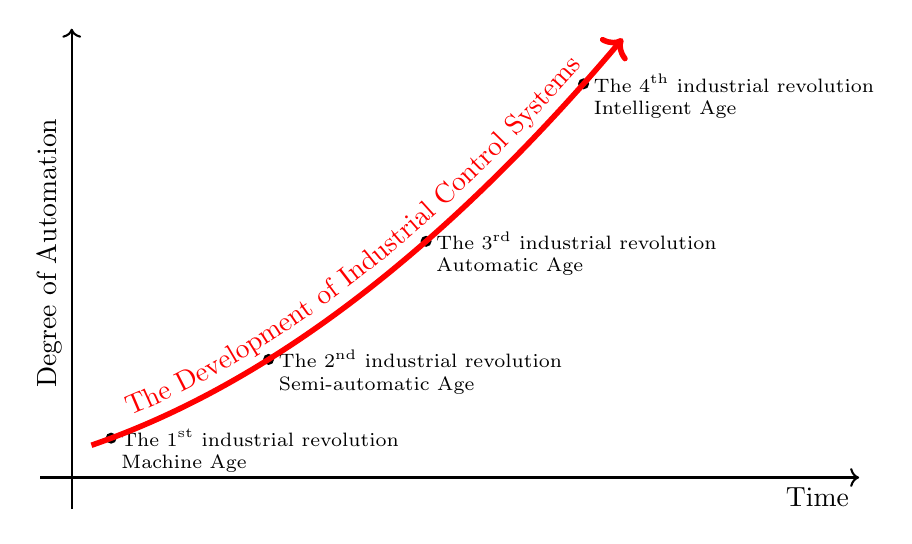
\begin{tikzpicture}[line width = \pgfdefaultlinewidth,
                    revolution/.style = {align = left, below = 4.5pt, right, font = \scriptsize}]

    \draw[->] (-0.4,0) -- (0,0) -- (10,0) node [anchor = north east] {Time};
    \draw[->] (0,-0.4) -- (0,0) -- (0,5.7) node [midway,sloped,above] {Degree of Automation};

    \coordinate (A) at (0.5, 0.5);
    \coordinate (B) at (2.5, 1.5);
    \coordinate (C) at (4.5, 3.0);
    \coordinate (D) at (6.5, 5.0);


    \fill (A) circle (2pt) node [revolution] {The 1\textsuperscript{st} industrial revolution\\Machine Age};
    \pause
    \fill (B) circle (2pt) node [revolution] {The 2\textsuperscript{nd} industrial revolution\\Semi-automatic Age};
    \pause
    \fill (C) circle (2pt) node [revolution] {The 3\textsuperscript{rd} industrial revolution\\Automatic Age};
    \pause
    \fill (D) circle (2pt) node [revolution] {The 4\textsuperscript{th} industrial revolution\\Intelligent Age};

    \pause
    \draw[postaction={decoration={text along path, transform={yshift=5pt}, text color=red, text={The Development of Industrial Control Systems},
text align=center}, decorate}]
    [domain=0.25:7, variable=\x, samples=200, ->, red, line width = 2pt] plot({\x},{(0.0625*\x^2 + 0.3125*\x + 0.3281)});
    
    
    
    
\end{tikzpicture} 
    \end{center}
\end{frame}

\begin{frame}{Background}\label{Introduction: ICSs are Important}
    \begin{itemize}
      \item ICSs have been widely applied in various industry of the national economy and people's livelihood, and gradually become the brain and central nervous of critical infrastructure and all kinds of industrial production.
      \item Once abnormal situation appears in ICSs , serious accidents may be happen, which may cause damage to property, people or a wide range of environment.
    \end{itemize}

    \begin{center}
      \begin{minipage}[m]{0.9\textwidth}
        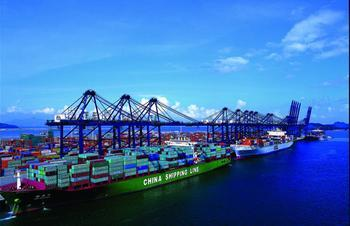
\includegraphics[height=1.5cm]{Figures/Introduction/Fig1.png} \hfill
        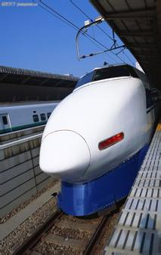
\includegraphics[height=1.5cm]{Figures/Introduction/Fig2.png} \hfill
        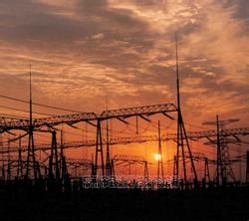
\includegraphics[height=1.5cm]{Figures/Introduction/Fig3.png} \hfill
        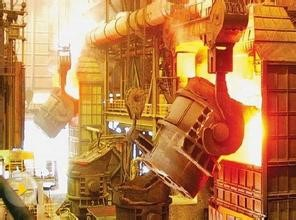
\includegraphics[height=1.5cm]{Figures/Introduction/Fig4.png} \hfill
        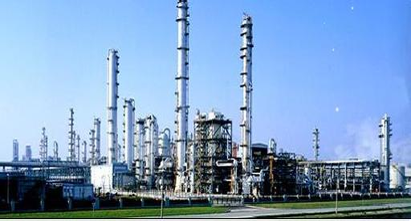
\includegraphics[height=1.5cm]{Figures/Introduction/Fig5.png} \vspace{1pt}\\
        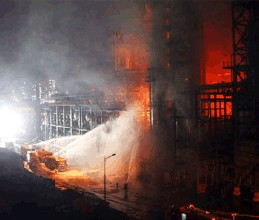
\includegraphics[height=1.5cm, width = 2.2cm]{Figures/Introduction/Fig6.png} \hfill
        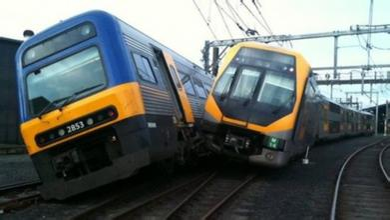
\includegraphics[height=1.5cm]{Figures/Introduction/Fig7.png} \hfill
        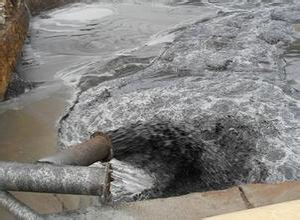
\includegraphics[height=1.5cm]{Figures/Introduction/Fig8.png} \hfill
        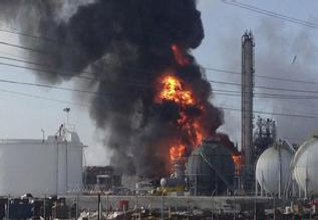
\includegraphics[height=1.5cm]{Figures/Introduction/Fig9.png}
      \end{minipage}
    \end{center}
\end{frame}

\begin{frame}{Background}\label{Introduction: ICSs are under Attacks}
    \begin{itemize}
      \item In 2010, Stuxnet attacked Iran's nuclear power plants and ruined almost one-fifth of Iran's nuclear centrifuges.
      \item In 2013, Israel Haifa highway control system  was attacked by hackers, which caused massive traffic congestion in the city which lead great loss and serious subsequent problems.
      \item In 2014, Havex malware infects many industrial control system in European  and caused the leakage of large amounts of data.
    \end{itemize}

    \begin{minipage}[c][][t]{0.6\textwidth}
      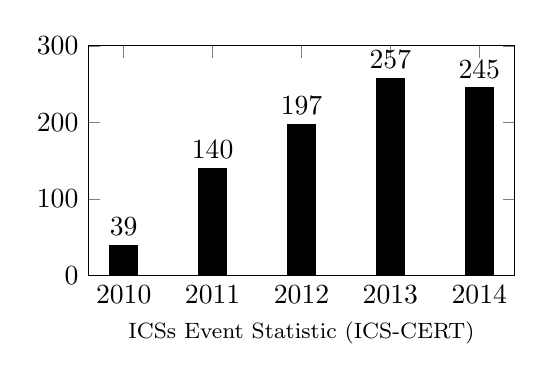
\begin{tikzpicture}[line width = \pgfdefaultlinewidth]

    \begin{axis}[symbolic x coords={2010, 2011, 2012, 2013, 2014},
                 xtick=data,
                 xlabel = {\footnotesize ICSs Event Statistic (ICS-CERT)},
                 width = 7cm,
                 height = 4.5cm,
                 nodes near coords,
                 ymax = 300,
                 ymin = 0]
        \addplot[ybar,fill=black] coordinates {
            (2010,39)
            (2011,140)
            (2012,197)
            (2013,257)
            (2014,245)
    };
\end{axis}
\end{tikzpicture} 
    \end{minipage}
    \begin{minipage}[c][][t]{0.35\textwidth}
    \begin{tikzpicture}
      \node (A) at (0,1.5) {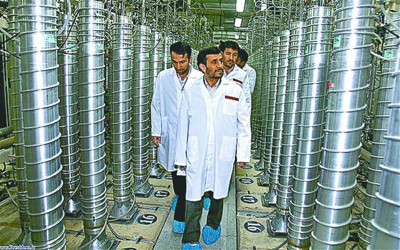
\includegraphics[height=2.2cm]{Figures/Introduction/Fig10.png}};
      \node[line width = 3pt, draw = white, inner sep=0pt] (B) at (1,0) {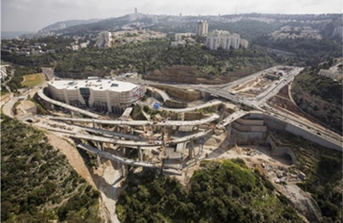
\includegraphics[height=2.2cm]{Figures/Introduction/Fig11.png}};
    \end{tikzpicture}
    \end{minipage}
\end{frame}

\begin{frame}{Problems -- Timeliness and Availability}\label{Introduction: Problem of Timeliness and Availability}
    ICSs have rigorous requirements on timeliness and availability. The cybersecurity risks of ICSs are primarily from the potential loss caused by the cyber-attacks which demolish the timeliness and availability of the control system.
    
    \pause
    In order to achieve the destructive purpose, attackers generally need to follow part or all of these three steps:
    \begin{enumerate}
      \item infiltrate into the field network,
      \item invalidate the system functions,
      \item cause the hazardous incidents.
    \end{enumerate}

    \pause
    Therefore, the cybersecurity risk assessment of ICSs needs  a novel and targeted risk model to analyze the risk propagation.
\end{frame}

\begin{frame}{Problems -- Overlapping amongst Consequences}\label{Introduction: Problem of Overlapping amongst Consequences}
    The majority of existing quantitative risk assessment approaches used the following definition to calculate the risk $\risk$.
    \[
        \risk = \sum_i S(e_i)P(e_i)
    \]
    
    \pause
    However, the overlapping amongst difference consequences may cause the error of risk value. \pause For example,
    \vspace{10pt}\\
    \begin{minipage}[l]{0.2\textwidth}
      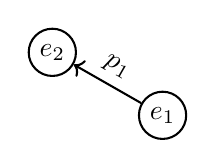
\begin{tikzpicture}[line width = \pgfdefaultlinewidth,
                    incident/.style = {draw, circle, inner sep = 0pt, align = center, minimum size = 0.6cm},
                    tag/.style = {align = right, anchor = west}]

    \node[incident] (e1) at (1.4,0.1) {$e_1$};
    \node[incident] (e2) at (0,0.9) {$e_2$};

    \draw[->] (e1) -- (e2) node[midway, above, sloped] {$p_1$};

   % \node[tag] at (1.7,1)   {Incident $e_1$ is the temperature anomaly of reactor,};
%    \node[tag] at (1.7,0.5) {incident $e_2$ is the explosion of reactor,};
%    \node[tag] at (1.7,0)   {when $e_1$ or $e_2$ happens, the product will be damaged.};
\end{tikzpicture} 
    \end{minipage}
    \begin{minipage}[l]{0.8\textwidth}
        incident $e_1$ is the temperature anomaly of reactor, incident $e_2$ is the explosion of reactor, when $e_1$ or $e_2$ happens, the product will be damaged.
    \end{minipage}
    \vspace{10pt}\\\pause
    Assume that $P(e_1) = 1$, so $P(e_2) = p_1$, then
    \[
        \risk = S(e_1) + p_1S(e_2) = S(e_1) + p_1S(e_1) = (1+p_1)S(e_1) \geq S(e_1)\text{.}
    \]
\end{frame}

\begin{frame}{Problems -- Unknown Attacks}\label{Introduction: Problem of Unknown Attacks}
    Many ICSs run 24/7/365, and therefore the updates must be planned and scheduled days or weeks in advance. After the updates, exhaustive testing is necessary to ensure the high availability of the ICS.
    
    \pause
    This leads to inability of the attack knowledge of ICSs to be updated in time. Several attack knowledge-based risk assessments cannot work well on ICSs.

    \pause
    Therefore, the risk assessment should have the ability of assessing the risk caused by unknown attacks without the corresponding attack knowledge.
\end{frame} 
\section{Architecture}
\begin{frame}{Architecture of Cybersecurity Risk Assessment for ICSs}
    \begin{center}
        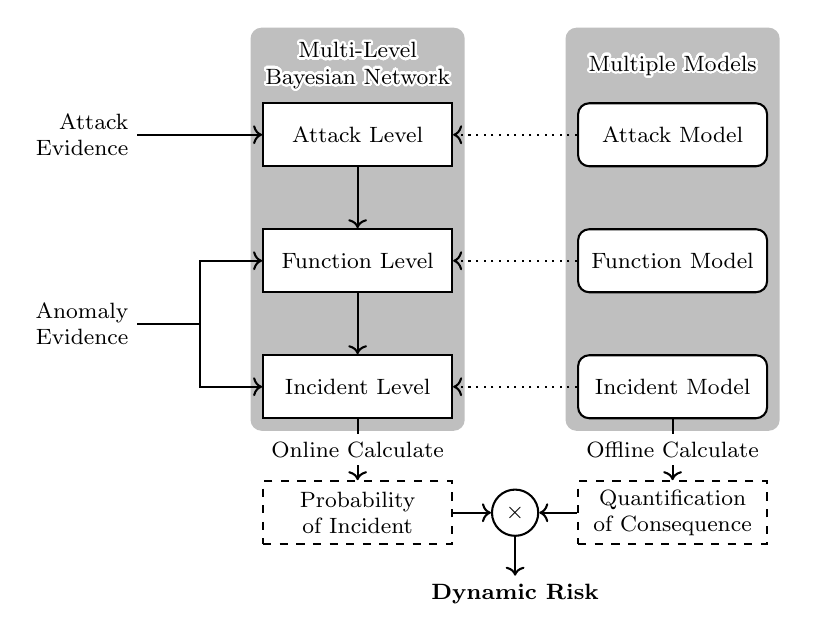
\begin{tikzpicture}[line width = \pgfdefaultlinewidth,
                    x = 0.8cm,
                    y = 0.8cm,
                    layer/.style = {fill = white, draw, rectangle, minimum height = 0.8cm, minimum width = 2.4cm, align = center, inner sep = 0pt},
	                model/.style = {fill = white, draw, rectangle, minimum height = 0.8cm, minimum width = 2.4cm, align = center, inner sep = 0pt, rounded corners},
	                value/.style = {draw, dashed, rectangle, minimum height = 0.8cm, minimum width = 2.4cm, align = center, inner sep = 0pt}]

\footnotesize

\fill[lightgray, rounded corners] (7.3, 3.3) rectangle (10.7, 9.7);
\node at (9,9.1) [text shadow={[align=center,text width=3cm] at (9,9.1) {Multiple Models}}] {Multiple Models};
\node (AM) at (9,8) [model] {Attack Model};
\node (FM) at (9,6) [model] {Function Model};
\node (IM) at (9,4) [model] {Incident Model};
\pause

\fill[lightgray, rounded corners] (2.3, 3.3) rectangle (5.7, 9.7);
\node at (4,9.1) [text shadow={[align=center,text width=3cm] at (4,9.1) {Multi-Level Bayesian Network}}] {Multi-Level Bayesian Network};
\node (AL) at (4,8) [layer] {Attack Level};
\node (FL) at (4,6) [layer] {Function Level};
\node (IL) at (4,4) [layer] {Incident Level};

\draw[dotted, ->] (AM) -- (AL);
\draw[dotted, ->] (FM) -- (FL);
\draw[dotted, ->] (IM) -- (IL);

\draw[->] (AL) -- (FL);
\draw[->] (FL) -- (IL);
\pause

\node (AT) at (0.5,8) [anchor = east, align = right] {Attack\\Evidence};
\node (AN) at (0.5,5) [anchor = east, align = right] {Anomaly\\Evidence};
\pause

\draw[->] (AT) -- (AL);
\pause

\draw[->] (AN) -- (1.5,5) |- (FL);
\draw[->] (1.5,5) |- (IL);
\pause

\node (IP) at (4,2) [value] {Probability\\of Incident};
\draw[->] (IL) -- (IP);
\node at (4,3) [fill = white] {Online Calculate};
\pause

\node (CQ) at (9,2) [value] {Quantification\\of Consequence};
\draw[->] (IM) -- (CQ);
\node at (9,3) [fill = white] {Offline Calculate};
\pause

\node (TI) at (6.5,2) [circle, draw] {$\times$};
\draw[->] (CQ) -- (TI);
\draw[->] (IP) -- (TI);
\pause

\draw[->] (TI) -- (6.5,1) node [anchor = north, align = center] {\textbf{Dynamic Risk}};

\onslide<1->
\end{tikzpicture} 
    \end{center}
\end{frame}
\section{Hazardous Incident Prediction}
\subsection{The Bayesian Network Based Knowledge Modeling}
\begin{frame}{Attack Level}
    In this paper, the Bayesian network is used to model the relationship between attacks and resources.
    \begin{center}
      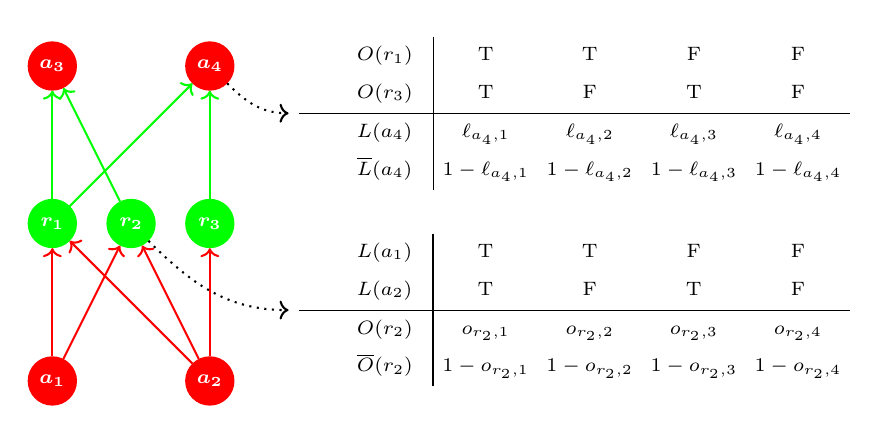
\begin{tikzpicture}[line width = \pgfdefaultlinewidth,
                    attack/.style = {draw = red, fill = red, text = white, circle, font = \scriptsize, minimum size = 0.6cm, inner sep = 0pt},
                    resource/.style = {draw = green, fill = green, text = white, circle, font = \scriptsize, minimum size = 0.6cm, inner sep = 0pt}]

    \pgfmathsetmacro{\interval}{2}

    
    \node[attack] (a1) at (1, 0*\interval) {$\bm{a_1}$};
    \node[attack] (a2) at (3, 0*\interval) {$\bm{a_2}$};
    \pause

    \node[resource] (r1) at (1, 1*\interval) {$\bm{r_1}$};
    \node[resource] (r2) at (2, 1*\interval) {$\bm{r_2}$};
    \node[resource] (r3) at (3, 1*\interval) {$\bm{r_3}$};

    \foreach \i/\j in{1/1,
                      1/2,
                      2/1,
                      2/2,
                      2/3}
    {
        \draw[->, red] (a\i) -- (r\j);
    }
    \pause


    \node[attack] (a3) at (1, 2*\interval) {$\bm{a_3}$};
    \node[attack] (a4) at (3, 2*\interval) {$\bm{a_4}$};

    \foreach \i/\j in {1/3,
                       1/4,
                       2/3,
                       3/4}
    {
        \draw[->, green] (r\i) -- (a\j);
    }
    \pause

    \extrarowsep =1mm
    \node[anchor = north west] (CPTR2) at (4,2) {\scriptsize
        \begin{tabu}to 7cm{X[l,-1]@{}|@{}*4{X[c,-1]@{}}}

            $L(a_1)$ & T & T & F & F\\
            $L(a_2)$ & T & F & T & F \\
            \hline
            $O(r_2)$ & $o_{r_2,1}$ & $o_{r_2,2}$ & $o_{r_2,3}$ & $o_{r_2,4}$\\
            $\overline{O}(r_2)$ & $1-o_{r_2,1}$ & $1-o_{r_2,2}$ & $1-o_{r_2,3}$ & $1-o_{r_2,4}$
        \end{tabu}
    };
    \draw[->, dotted] (r2) to[out=-45, in=180] (CPTR2);
    \pause

    \node[anchor = north west] (CPTA4) at (4,4.5) {\scriptsize
        \begin{tabu}to 7cm{X[l,-1]@{}|@{}*4{X[c,-1]@{}}}

            $O(r_1)$ & T & T & F & F\\
            $O(r_3)$ & T & F & T & F\\
            \hline
            $L(a_4)$ & $\ell_{a_4,1}$ & $\ell_{a_4,2}$ & $\ell_{a_4,3}$ & $\ell_{a_4,4}$\\
            $\overline{L}(a_4)$ & $1-\ell_{a_4,1}$ & $1-\ell_{a_4,2}$ & $1-\ell_{a_4,3}$ & $1-\ell_{a_4,4}$
        \end{tabu}
    };
    \draw[->, dotted] (a4) to[out=-45, in=180] (CPTA4);


    \onslide<1->
\end{tikzpicture} 
    \end{center}

\end{frame}

\begin{frame}{Function Level}
    Function Tree Analysis is widely used to analyze the stability of control system, a typical function tree is shown in following figure.
    \begin{center}
      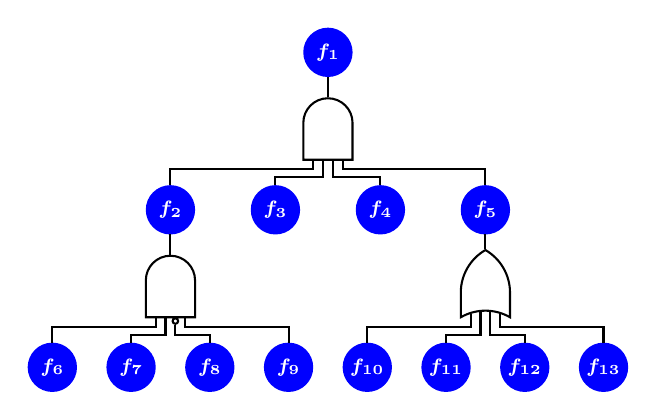
\begin{tikzpicture}[line width = \pgfdefaultlinewidth,
                    circuit logic US,
                    function/.style = {draw = blue, fill = blue, text = white, circle, font = \scriptsize, minimum size = 0.6cm, inner sep = 0pt}]
    \pause
    \node[function] (f1)  at (3.5,4) {$\bm{f_{1}}$};
    \pause
    \pause

    \node[and gate,point up,logic gate inputs=1234,logic gate inverted radius=1pt] (gate1) at (3.5,3) {};
    \draw (gate1.output) -- (f1);

    \node[function] (f2)  at (1.5,2) {$\bm{f_2}$};
    \node[function] (f3) at (1.5+4/3,2) {$\bm{f_{3}}$};
    \node[function] (f4) at (1.5+8/3,2) {$\bm{f_{4}}$};
    \node[function] (f5) at (5.5,2) {$\bm{f_{5}}$};

    \draw (f2.north) -- ++ (up:2mm) -| (gate1.input 1);
    \draw (f3.north) -- ++ (up:1mm) -| (gate1.input 2);
    \draw (f4.north) -- ++ (up:1mm) -| (gate1.input 3);
    \draw (f5.north) -- ++ (up:2mm) -| (gate1.input 4);

    \pause
    \pause

    \node[and gate,point up,logic gate inputs=nnin, logic gate inverted radius=1pt] (gate2) at (1.5,1) {};
    \draw (gate2.output) -- (f2);

    \node[function] (f6) at (0,0) {$\bm{f_6}$};
    \node[function] (f7) at (1,0) {$\bm{f_7}$};
    \node[function] (f8) at (2,0) {$\bm{f_8}$};
    \node[function] (f9) at (3,0) {$\bm{f_9}$};

    \draw (f6.north) -- ++ (up:2mm) -| (gate2.input 1);
    \draw (f7.north) -- ++ (up:1mm) -| (gate2.input 2);
    \draw (f8.north) -- ++ (up:1mm) -| (gate2.input 3);
    \draw (f9.north) -- ++ (up:2mm) -| (gate2.input 4);

    \pause
    \pause

    \node[or gate,point up,logic gate inputs=1234,logic gate inverted radius=1pt] (gate3) at (5.5,1) {};
    \draw (gate3.output) -- (f5);

    \node[function] (f10) at (4,0) {$\bm{f_{10}}$};
    \node[function] (f11) at (5,0) {$\bm{f_{11}}$};
    \node[function] (f12) at (6,0) {$\bm{f_{12}}$};
    \node[function] (f13) at (7,0) {$\bm{f_{13}}$};

    \draw (f10.north) -- ++ (up:2mm) -| (gate3.input 1);
    \draw (f11.north) -- ++ (up:1mm) -| (gate3.input 2);
    \draw (f12.north) -- ++ (up:1mm) -| (gate3.input 3);
    \draw (f13.north) -- ++ (up:2mm) -| (gate3.input 4);

    \onslide<1->
\end{tikzpicture} 
    \end{center}

    \begin{overlayarea}{\textwidth}{1cm}
    \only<3-4>{
        \[
            F_1 = F_2F_3F_4F_5
        \]
    }
    \only<5-6>{
        \[
            F_2 = F_6F_7\overline{F_8}F_9
        \]
    }
    \only<7-8>{
        \[
            F_5 = F_{10}+F_{11}+F_{12}+F_{13}
        \]
    }
    \end{overlayarea}
\end{frame}

\begin{frame}{Function Level}
    To simplify the inference, the function tree is converted into Bayesian network, which is shown in following figure.\\
    \begin{overlayarea}{\textwidth}{6cm}
    \begin{center}
      \only<1-3>{
        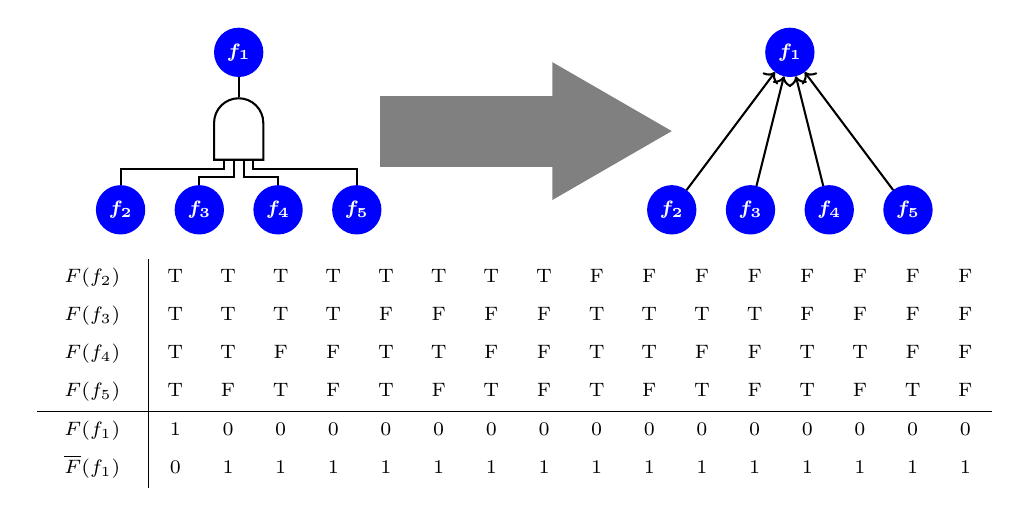
\begin{tikzpicture}[line width = \pgfdefaultlinewidth,
                    circuit logic US,
                    function/.style = {draw = blue, fill = blue, text = white, circle, font = \scriptsize, minimum size = 0.6cm, inner sep = 0pt}]

    \node[function] (f1) at (2.5,4) {$\bm{f_{1}}$};

    \node[and gate,point up,logic gate inputs=1234,logic gate inverted radius=1pt] (gate1) at (2.5,3) {};
    \draw (gate1.output) -- (f1);

    \node[function] (f2) at (1,2) {$\bm{f_2}$};
    \node[function] (f3) at (2,2) {$\bm{f_{3}}$};
    \node[function] (f4) at (3,2) {$\bm{f_{4}}$};
    \node[function] (f5) at (4,2) {$\bm{f_{5}}$};

    \draw (f2.north) -- ++ (up:2mm) -| (gate1.input 1);
    \draw (f3.north) -- ++ (up:1mm) -| (gate1.input 2);
    \draw (f4.north) -- ++ (up:1mm) -| (gate1.input 3);
    \draw (f5.north) -- ++ (up:2mm) -| (gate1.input 4);


    \node[function] (f1') at (9.5,4) {$\bm{f_{1}}$};

    \node[function] (f2') at (8,2) {$\bm{f_2}$};
    \node[function] (f3') at (9,2) {$\bm{f_3}$};
    \node[function] (f4') at (10,2) {$\bm{f_4}$};
    \node[function] (f5') at (11,2) {$\bm{f_5}$};

    \path[draw=black!50,solid,line width=9mm,fill=black!50, preaction={-triangle 60,line width = 4mm,draw = black!50,shorten >=-10mm}] (4.3,3) -- (7,3);

    \draw[->] (f2') -- (f1');
    \draw[->] (f3') -- (f1');
    \draw[->] (f4') -- (f1');
    \draw[->] (f5') -- (f1');

    \extrarowsep =1mm
    \node[anchor = north] (CPT) at (6,1.5) {\scriptsize
        \begin{tabu}{X[4,c]|*{16}{X[c]}}
          $F(f_2)$ & T & T & T & T & T & T & T & T & F & F & F & F & F & F & F & F \\
          $F(f_3)$ & T & T & T & T & F & F & F & F & T & T & T & T & F & F & F & F \\
          $F(f_4)$ & T & T & F & F & T & T & F & F & T & T & F & F & T & T & F & F \\
          $F(f_5)$ & T & F & T & F & T & F & T & F & T & F & T & F & T & F & T & F \\
          \hline
          $F(f_1)$ & $1$ & $0$ & $0$ & $0$ & $0$ & $0$ & $0$ & $0$ & $0$ & $0$ & $0$ & $0$ & $0$ & $0$ & $0$ & $0$ \\
          $\overline{F}(f_1)$ & $0$ & $1$ & $1$ & $1$ & $1$ & $1$ & $1$ & $1$ & $1$ & $1$ & $1$ & $1$ & $1$ & $1$ & $1$ & $1$
        \end{tabu}
    };

    \onslide<1->
\end{tikzpicture} 
      }
      \only<4-6>{
        \begin{tikzpicture}[line width = \pgfdefaultlinewidth,
                    circuit logic US,
                    function/.style = {draw = blue, fill = blue, text = white, circle, font = \scriptsize, minimum size = 0.6cm, inner sep = 0pt}]

    \node[function] (f2) at (2.5,4) {$\bm{f_{2}}$};

    \node[and gate,point up,logic gate inputs=nnin,logic gate inverted radius=1pt] (gate1) at (2.5,3) {};
    \draw (gate1.output) -- (f1);

    \node[function] (f6) at (1,2) {$\bm{f_6}$};
    \node[function] (f7) at (2,2) {$\bm{f_{7}}$};
    \node[function] (f8) at (3,2) {$\bm{f_{8}}$};
    \node[function] (f9) at (4,2) {$\bm{f_{9}}$};

    \draw (f6.north) -- ++ (up:2mm) -| (gate1.input 1);
    \draw (f7.north) -- ++ (up:1mm) -| (gate1.input 2);
    \draw (f8.north) -- ++ (up:1mm) -| (gate1.input 3);
    \draw (f9.north) -- ++ (up:2mm) -| (gate1.input 4);
    \pause\pause\pause\pause

    \path[draw=black!50,solid,line width=9mm,fill=black!50, preaction={-triangle 60,line width = 4mm,draw = black!50,shorten >=-10mm}] (4.3,3) -- (7,3);
    \node[text shadow={[align=center,text width=3cm] at (5.7,3) {Convert}}] at (5.7,3) {Convert};

    \node[function] (f2') at (9.5,4) {$\bm{f_{2}}$};

    \node[function] (f6') at (8,2) {$\bm{f_6}$};
    \node[function] (f7') at (9,2) {$\bm{f_7}$};
    \node[function] (f8') at (10,2) {$\bm{f_8}$};
    \node[function] (f9') at (11,2) {$\bm{f_9}$};

    \draw[->] (f6') -- (f2');
    \draw[->] (f7') -- (f2');
    \draw[->] (f8') -- (f2');
    \draw[->] (f9') -- (f2');
    \pause

    \extrarowsep =1mm
    \node[anchor = north] (CPT) at (6,1.5) {\scriptsize
        \begin{tabu}{X[4,c]|*{16}{X[c]}}
          $F(f_6)$ & T & T & T & T & T & T & T & T & F & F & F & F & F & F & F & F \\
          $F(f_7)$ & T & T & T & T & F & F & F & F & T & T & T & T & F & F & F & F \\
          $F(f_8)$ & T & T & F & F & T & T & F & F & T & T & F & F & T & T & F & F \\
          $F(f_9)$ & T & F & T & F & T & F & T & F & T & F & T & F & T & F & T & F \\
          \hline
          $F(f_1)$ & $1$ & $1$ & $0$ & $1$ & $1$ & $1$ & $1$ & $1$ & $1$ & $1$ & $1$ & $1$ & $1$ & $1$ & $1$ & $1$ \\
          $\overline{F}(f_1)$ & $0$ & $0$ & $1$ & $0$ & $0$ & $0$ & $0$ & $0$ & $0$ & $0$ & $0$ & $0$ & $0$ & $0$ & $0$ & $0$
        \end{tabu}
    };

    \onslide<1->
\end{tikzpicture} 
      }
      \only<7-9>{
        \begin{tikzpicture}[line width = \pgfdefaultlinewidth,
                    circuit logic US,
                    function/.style = {draw = blue, fill = blue, text = white, circle, font = \scriptsize, minimum size = 0.6cm, inner sep = 0pt}]

    \node[function] (f5) at (2.5,4) {$\bm{f_{5}}$};

    \node[or gate,point up,logic gate inputs=nnnn,logic gate inverted radius=1pt] (gate1) at (2.5,3) {};
    \draw (gate1.output) -- (f1);

    \node[function] (f10) at (1,2) {$\bm{f_{10}}$};
    \node[function] (f11) at (2,2) {$\bm{f_{11}}$};
    \node[function] (f12) at (3,2) {$\bm{f_{12}}$};
    \node[function] (f13) at (4,2) {$\bm{f_{13}}$};

    \draw (f10.north) -- ++ (up:2mm) -| (gate1.input 1);
    \draw (f11.north) -- ++ (up:1mm) -| (gate1.input 2);
    \draw (f12.north) -- ++ (up:1mm) -| (gate1.input 3);
    \draw (f13.north) -- ++ (up:2mm) -| (gate1.input 4);
    \pause\pause\pause\pause\pause\pause\pause
    
    \path[draw=black!50,solid,line width=9mm,fill=black!50, preaction={-triangle 60,line width = 4mm,draw = black!50,shorten >=-10mm}] (4.3,3) -- (7,3);
    \node[text shadow={[align=center,text width=3cm] at (5.7,3) {Convert}}] at (5.7,3) {Convert};
    \node[function] (f5') at (9.5,4) {$\bm{f_{5}}$};

    \node[function] (f10') at (8,2) {$\bm{f_{10}}$};
    \node[function] (f11') at (9,2) {$\bm{f_{11}}$};
    \node[function] (f12') at (10,2) {$\bm{f_{12}}$};
    \node[function] (f13') at (11,2) {$\bm{f_{13}}$};

    \draw[->] (f10') -- (f5');
    \draw[->] (f11') -- (f5');
    \draw[->] (f12') -- (f5');
    \draw[->] (f13') -- (f5');
    \pause
    
    \extrarowsep =1mm
    \node[anchor = north] (CPT) at (6,1.5) {\scriptsize
        \begin{tabu}{X[4,c]|*{16}{X[c]}}
          $F(f_{10})$ & T & T & T & T & T & T & T & T & F & F & F & F & F & F & F & F \\
          $F(f_{11})$ & T & T & T & T & F & F & F & F & T & T & T & T & F & F & F & F \\
          $F(f_{12})$ & T & T & F & F & T & T & F & F & T & T & F & F & T & T & F & F \\
          $F(f_{13})$ & T & F & T & F & T & F & T & F & T & F & T & F & T & F & T & F \\
          \hline
          $F(f_5)$ & $1$ & $0$ & $0$ & $0$ & $0$ & $0$ & $0$ & $0$ & $0$ & $0$ & $0$ & $0$ & $0$ & $0$ & $0$ & $0$ \\
          $\overline{F}(f_5)$ & $0$  & $1$ & $1$ & $1$ & $1$ & $1$ & $1$ & $1$ & $1$ & $1$ & $1$ & $1$ & $1$ & $1$& $1$ & $1$
        \end{tabu}
    };
    \onslide<1->
\end{tikzpicture} 
      }
    \end{center}
    \end{overlayarea}
\end{frame}

\begin{frame}{Function Level}
    \uncover<4>{The conditional probability table of the Bayesian network contains more information than the logical gate of the fault tree.\\}
    \begin{overlayarea}{\textwidth}{6cm}
    \begin{center}
      \begin{tikzpicture}[line width = \pgfdefaultlinewidth,
                    circuit logic US,
                    function/.style = {draw = blue, fill = blue, text = white, circle, font = \scriptsize, minimum size = 0.6cm, inner sep = 0pt}]
    \node[function] (f1) at (9.5,4) {$\bm{f_{1}}$};

    \node[and gate,point up,logic gate inputs=1234,logic gate inverted radius=1pt] (gate1) at (9.5,3) {};
    \draw (gate1.output) -- (f1);

    \node[function] (f2) at (8,2) {$\bm{f_2}$};
    \node[function] (f3) at (9,2) {$\bm{f_{3}}$};
    \node[function] (f4) at (10,2) {$\bm{f_{4}}$};
    \node[function] (f5) at (11,2) {$\bm{f_{5}}$};

    \draw (f2.north) -- ++ (up:2mm) -| (gate1.input 1);
    \draw (f3.north) -- ++ (up:1mm) -| (gate1.input 2);
    \draw (f4.north) -- ++ (up:1mm) -| (gate1.input 3);
    \draw (f5.north) -- ++ (up:2mm) -| (gate1.input 4);

    \path[draw=black!50,solid,line width=9mm,fill=black!50, preaction={-triangle 60,line width = 4mm,draw = black!50,shorten >=-10mm}] (4.3,3) -- (7,3);
    \node[text shadow={[align=center,text width=3cm] at (5.7,3) {Convert}}] at (5.7,3) {Convert};

    \only<1-2| trans:1>{
        \node[text = red] at (5.7,3) {\scalebox{7}{\Black ?}};
    }
    \only<3-| trans:2>{
        \node[forbidden sign,text width=1.5cm, text centered, draw = red, line width = 8pt] at (5.7,3) {};
    }

    \node[function] (f1') at (2.5,4) {$\bm{f_{1}}$};

    \node[function] (f2') at (1,2) {$\bm{f_2}$};
    \node[function] (f3') at (2,2) {$\bm{f_3}$};
    \node[function] (f4') at (3,2) {$\bm{f_4}$};
    \node[function] (f5') at (4,2) {$\bm{f_5}$};

    \draw[->] (f2') -- (f1');
    \draw[->] (f3') -- (f1');
    \draw[->] (f4') -- (f1');
    \draw[->] (f5') -- (f1');
    \pause

    \extrarowsep =1mm
    \node[anchor = north] (CPT) at (6,1.5) {\scriptsize
        \begin{tabu}{X[4,c]|*{16}{X[c]}}
          $F(f_2)$ & T & T & T & T & T & T & T & T & F & F & F & F & F & F & F & \textcolor{red}{\textbf{F}} \\
          $F(f_3)$ & T & T & T & T & F & F & F & F & T & T & T & T & F & F & F & \textcolor{red}{\textbf{F}} \\
          $F(f_4)$ & T & T & F & F & T & T & F & F & T & T & F & F & T & T & F & \textcolor{red}{\textbf{F}} \\
          $F(f_5)$ & T & F & T & F & T & F & T & F & T & F & T & F & T & F & T & \textcolor{red}{\textbf{F}} \\
          \hline
          $F(f_1)$ & $1$ & $1$ & $1$ & $1$ & $1$ & $1$ & $1$ & $1$ & $1$ & $1$ & $1$ & $1$ & $1$ & $1$ & $1$ & \textcolor{red}{$\mathclap{\bm{0.5}}$} \\
          $\overline{F}(f_1)$ & $0$ & $0$ & $0$ & $0$ & $0$ & $0$ & $0$ & $0$ & $0$ & $0$ & $0$ & $0$ & $0$ & $0$ & $0$ & \textcolor{red}{$\mathclap{\bm{0.5}}$}
        \end{tabu}
    };

    \onslide<1->
\end{tikzpicture} 
    \end{center}
    \end{overlayarea}
\end{frame}

\begin{frame}{Incident Level}
\end{frame}

\subsection{Incident Prediction}
\begin{frame}{Collection of Evidence}
\end{frame}

\begin{frame}{Calculation of Incident Probability}
\end{frame} 
\label{Section: Dynamic Risk Assessment}
\section{Dynamic Risk Assessment}
\subsection{Decouple of Incident Consequences}
\begin{frame}{Decouple of Incident Consequences -- Step 1}
    \label{Dynamic Risk Assessment: Decouple of Incident Consequences Step 1}
    For each incident $e_i$, analyze its consequence and generate a consequence set
    \[
        \bm{c}_i = (c_1, c_2, \cdots, c_n) \text{.}
    \]

    The meaning of $\bm{c}_i$ is that the occurring of the incident $e_i$ will threaten the elements in consequence set $\bm{c}_i$.\\[10pt]

    For example, the incident $e_i$ is an explosion of a reactor, which may cause worker casualties, air pollution, facilities damages, and products loss. The consequence set of $e_i$ is
    \[
    \bm{c}_i = (\text{workers}, \text{air}, \text{facilities}, \text{products})\text{.}
    \]
\end{frame}

\begin{frame}{Decouple of Incident Consequences -- Step 2}
    \label<trans:1>{Dynamic Risk Assessment: Decouple of Incident Consequences Step 2 Conditions}
    \label<trans:2>{Dynamic Risk Assessment: Decouple of Incident Consequences Step 2 Example}
    Then, generate $\bm{C}' = (\bm{c}_1',\bm{c}_2',\cdots,\bm{c}_{m'}')$ based on $\bm{C} = (\bm{c}_1, \bm{c}_2, \cdots, \bm{c}_m)$. The following conditions must be met:
    \begin{align}
        \text{Completeness: } & \textstyle\bigcup_{i=1}^m \bm{c}_i= \bigcup_{i=1}^{m'} \bm{c}_i'\text{,}\notag\\
        \text{Independence: } & \forall \bm{c}_i',\bm{c}_j' \in \bm{C}' \text{ : } \bm{c}_i' \cap \bm{c}_j' = \varnothing\text{,}\notag\\
        \text{Traceability: } & \forall \bm{c}' \in \bm{C}', \exists \bm{c} \in \bm{C} \text{ : } \bm{c}' \subseteq \bm{c}\text{.}\notag
    \end{align}
    \vspace{-30pt}
    \uncover<2-| trans:2>{
        \begin{center}
          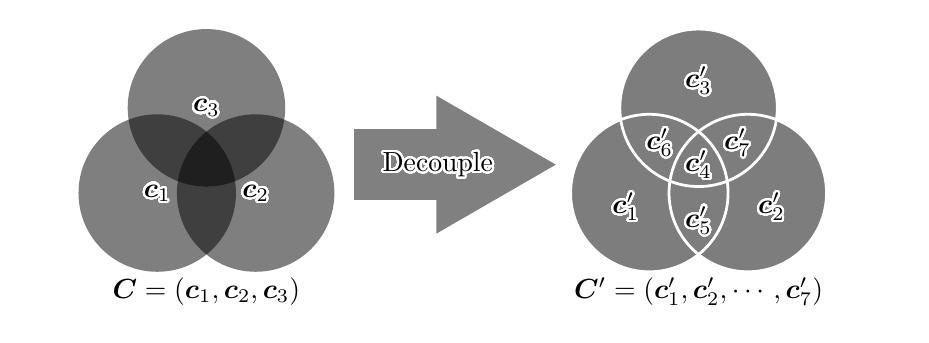
\begin{tikzpicture}[line width = \pgfdefaultlinewidth,
                    x = 0.625cm,
                    y = 0.625cm]

    \pgfmathsetmacro{\distance}{10}

    \node at (3,0) {
    $\bm{C} = (     \pause
        \bm{c}_1,   \pause
        \bm{c}_2,   \pause
        \bm{c}_3)$
    };

    \uncover<2->{
        \fill[fill opacity=0.5] (2,    2) circle (1.6);
        \node at (2,    2) [text shadow={[align=center,text width=3cm] at (2,    2) {$\bm{c}_1$}}] {$\bm{c}_1$};
    }
    \uncover<3->{
        \fill[fill opacity=0.5] (4,    2) circle (1.6);
        \node at (4,    2) [text shadow={[align=center,text width=3cm] at (4,    2) {$\bm{c}_2$}}] {$\bm{c}_2$};
    }
    \uncover<4->{
        \fill[fill opacity=0.5] (3,3.732) circle (1.6);
        \node at (3,3.732) [text shadow={[align=center,text width=3cm] at (3,3.732) {$\bm{c}_3$}}] {$\bm{c}_3$};
    }


    \uncover<5->{
    \path[draw=black!50,solid,line width=9mm,fill=black!50, preaction={-triangle 60,line width = 4mm,draw = black!50,shorten >=-10mm}] (3 + 3,2.577) -- (3 - 4.5 + \distance,2.577);
    \node[text shadow={[align=center,text width=3cm] at (2.7    + 0.5*\distance,2.577) {Decouple}}] at (2.7    + 0.5*\distance,2.577) {Decouple};

    \fill[fill = black!51] (2 + \distance,    2) circle (1.6);
    \fill[fill = black!51] (4 + \distance,    2) circle (1.6);
    \fill[fill = black!51] (3 + \distance,3.732) circle (1.6);

    \draw[white, line width = 1pt] (2 + \distance,    2) circle (1.6);
    \draw[white, line width = 1pt] (4 + \distance,    2) circle (1.6);
    \draw[white, line width = 1pt] (3 + \distance,3.732) circle (1.6);

    \node at (1.52 + \distance,1.72 ) [text shadow={[align=center,text width=3cm] at (1.52 + \distance,1.72 ) {$\bm{c}_1'$}}] {$\bm{c}_1'$};
    \node at (4.48 + \distance,1.72 ) [text shadow={[align=center,text width=3cm] at (4.48 + \distance,1.72 ) {$\bm{c}_2'$}}] {$\bm{c}_2'$};
    \node at (3    + \distance,4.29 ) [text shadow={[align=center,text width=3cm] at (3    + \distance,4.29 ) {$\bm{c}_3'$}}] {$\bm{c}_3'$};
    \node at (3    + \distance,2.577) [text shadow={[align=center,text width=3cm] at (3    + \distance,2.577) {$\bm{c}_4'$}}] {$\bm{c}_4'$};
    \node at (3    + \distance,1.447) [text shadow={[align=center,text width=3cm] at (3    + \distance,1.447) {$\bm{c}_5'$}}] {$\bm{c}_5'$};
    \node at (2.21 + \distance,3.03 ) [text shadow={[align=center,text width=3cm] at (2.21 + \distance,3.03 ) {$\bm{c}_6'$}}] {$\bm{c}_6'$};
    \node at (3.79 + \distance,3.03 ) [text shadow={[align=center,text width=3cm] at (3.79 + \distance,3.03 ) {$\bm{c}_7'$}}] {$\bm{c}_7'$};

    \node at (3 + \distance,0) {$\bm{C}' = (\bm{c}'_1,\bm{c}'_2,\cdots,\bm{c}'_7)$};
    }

    \onslide<1->
\end{tikzpicture} 
        \end{center}
    }

\end{frame}

\begin{frame}{Decouple of Incident Consequences -- Step 3}
    \label{Dynamic Risk Assessment: Decouple of Incident Consequences Step 3}
    For each $\bm{c}'_j \in \bm{C}'$, generate a corresponding auxiliary node $x_j$. According to the \textbf{traceability} of $\bm{C}'$
    \[
    \forall \bm{c}' \in \bm{C}', \exists \bm{c} \in \bm{C}, \bm{c}' \subseteq \bm{c}\text{,}
    \]
    \vspace{-15pt}\\
    there must be a consequence set $\bm{c}_i \in \bm{C}$ , where $\bm{c}'_j \subseteq \bm{c}_i$. \pause So, for each $\bm{c}'_j \in \bm{C}'$, we can find the incident set
    \[
    \bm{e}_j = (e_{i_1},e_{i_2},\cdots,e_{i_n})\text{.}
    \]
    \vspace{-15pt}\\\pause
    For each incident $e_k$ of the incident set $\bm{e}_j$, the corresponding consequence set $\bm{c}_k$ satisfies the following condition:
    \[
    \bm{c}'_j \subseteq \bm{c}_k\text{.}
    \]
    \vspace{-15pt}\\\pause
    Therefore, the parent nodes of the auxiliary node $x_j$ are incident nodes $e_{i_1},e_{i_2},\cdots,e_{i_n}$.
\end{frame}

\begin{frame}{Decouple of Incident Consequences -- Step 4}
    \label{Dynamic Risk Assessment: Decouple of Incident Consequences Step 4}
    For each auxiliary node $x_j$, generate a conditional probability table. A typical conditional probability table of auxiliary node $x_j$ is shown as following table.\\[-15pt]
    \extrarowsep = 0.7mm
    \begin{center}
      \begin{tabu}to \textwidth{@{}X[c,2]@{}|*7{X[c]}@{}}
        $H(e_{i_1})$        & T & T & T & $\cdots$ & F & F & F\\
        $H(e_{i_2})$        & T & T & T & $\cdots$ & F & F & F\\
        $H(e_{i_3})$        & T & T & T & $\cdots$ & F & F & F\\
        $\vdots$            & $\vdots$ & $\vdots$ & $\vdots$ & $\ddots$ & $\vdots$ & $\vdots$ & $\vdots$\\
        $H(e_{i_{n-2}})$    & T & T & T & $\cdots$ & F & F & F\\
        $H(e_{i_{n-1}})$    & T & T & F & $\cdots$ & T & F & F\\
        $H(e_{i_n})$        & T & F & F & $\cdots$ & F & T & F\\
        \hline
        $H(x_j)$            & $1$ & $1$ & $1$ & $\cdots$ & $1$ & $1$ & $0$ \\
        $\overline{H}(x_j)$ & $0$ & $0$ & $0$ & $\cdots$ & $0$ & $0$ & $1$
      \end{tabu}
    \end{center}
\end{frame}

\subsection{Classification of Incident Consequences}
\begin{frame}{Classification of Incident Consequences}
    \label{Dynamic Risk Assessment: Classification of Incident Consequences}
    In the proposed approach, there are three main kinds of incident consequences to be considered:
    \begin{itemize}
      \item \textbf{Harm to Humans:}\\[-5pt]
      \begin{itemize}
        \item[-] temporary harm,
        \item[-] permanent disability,
        \item[-] fatality.
      \end{itemize}
      \item \textbf{Environmental Pollution:}\\[-5pt]
      \begin{itemize}
        \item[-] air pollution,
        \item[-] soil contamination,
        \item[-] water pollution.
      \end{itemize}
      \item \textbf{Property Loss:}\\[-5pt]
      \begin{itemize}
        \item[-] damage of materials,
        \item[-] damage of products,
        \item[-] damage of equipment.
      \end{itemize}
    \end{itemize}
\end{frame}

\subsection{Quantification of Incident Consequences}
\begin{frame}{Quantification of Incident Consequences}
    \label{Dynamic Risk Assessment: Quantification of Incident Consequences}
    \begin{itemize}
      \item \textbf{Harm to Humans $Q_H$:}\\
      If the decision-maker would like to increase the cost of an investment by $\Delta c$ to reduce the  probability of a fatality by $\Delta p$,
      \[
        Q_H = \Delta c/\Delta p\text{.}
      \]
      \item \textbf{Environmental Pollution $Q_E$:}\\
      The monetary loss of environmental pollution is defined as
      \[
        Q_E = {\it Penalty} + {\it Compensation} + {\it HarnessCost}\text{.}
      \]
      \item \textbf{Property Loss $Q_P$:}\\
      The cost of replacement is used to quantify the loss of property $Q_P$, such as the loss of  materials, products, and equipment.
    \end{itemize}
\end{frame}

\subsection{Calculation of Dynamic Risk}
\begin{frame}{Calculation of Dynamic Risk}
    \label{Dynamic Risk Assessment: Calculation of Dynamic Risk}
    Due to the following two reasons:
    \begin{itemize}
      \item there is no overlapping between the consequences of any two auxiliary nodes $x_i$ and $x_j$, $i\neq j$,
      \item the auxiliary nodes contain all the consequences of incidents,
    \end{itemize}

    the dynamic cybersecurity risk can be defined as
    \[
        \risk = \sum_{i=1}^{m'}p(x_i)q(x_i)\text{,}
    \]

    where
    \begin{itemize}
      \item $p(x_i)$ is the occurrence probability of the auxiliary node $x_i$,
      \item $q(x_i)$ is the monetary loss of the auxiliary node $x_i$.
    \end{itemize}

\end{frame} 
\label{Section: Simulation}
\section{Simulation}
\subsection{Simulation Platform}
\begin{frame}{Simulation Platform}
    \label{Simulation: Control Structure of Chemical Reactor}
    The simulation object is a chemical reactor whose control structure is shown as the following figure.\\[-10pt]
    \begin{center}
      \newcommand{\computer}{
\includegraphics[width=0.7cm]{Figures/Materials/Computer.pdf}}
\newcommand{\router}{
\includegraphics[width=0.7cm]{Figures/Materials/Router.pdf}}
\newcommand{\plc}{
\includegraphics[width=0.65cm]{Figures/Materials/PLC.pdf}}
\newcommand{\server}{
\includegraphics[width=0.52cm]{Figures/Materials/Server.pdf}}

\newcommand{\mydot}{,}


\newcommand{\bus}[3]{
	\draw[fill = white] (#1, #2 + 0.15) to[out = 180, in = 180] (#1, #2 - 0.15) -- (#1 + #3, #2 - 0.15) to[in = 0, out = 0] (#1 + #3, #2 + 0.15) -- cycle;
	\draw (#1 + #3, #2 + 0.1) to[out = 180, in = 180] (#1 + #3, #2 - 0.1) to[in = 0, out = 0] cycle;
}

\newcommand{\valve}[3]{
	\draw[fill = white] (#1,#2) -- (#1 - 0.25, #2 + 0.15) -- (#1 - 0.25, #2 - 0.15) -- (#1 + 0.25, #2 + 0.15) -- (#1 + 0.25, #2 - 0.15) -- (#1 ,#2) -- (#1, #2 + 0.2) -- (#1 - 0.2, #2 + 0.2) to[out = 45, in = 135] (#1 + 0.2, #2 + 0.2) -- (#1, #2 + 0.2);
	\node (v#3) at (#1,#2) [rectangle, minimum width = 0.3cm] {};
}

\begin{tikzpicture}[line width = \pgfdefaultlinewidth,
                    x = 0.6cm,
                    y = 0.6cm,
                    tag/.style = {pos = 0.7}]
\scriptsize

% Networks
\draw (2,9) node {\server} -- (2,8);
\draw (5,9) node {\computer} -- (5,8);
\draw (8,9.5) -- (8,9) node {\router} -- (8,8);
\draw (3.5,8) -- (3.5,7) node {\router} -- (3.5,6);
\draw (8,8) -- (8,7) node {\router} -- (8,6);

\foreach \i in {1,...,6}{
    \draw (1.5*\i + 0.5,6) -- (1.5*\i + 0.5,5) node {\plc} -- (1.5*\i + 0.5,4);
    \node [below = -8pt, text shadow={[align=center, below = -8pt] at (1.5*\i + 0.5,4) {PLC\i}}] at (1.5*\i + 0.5,4) {PLC\i};
}

% Water Level
\fill[blue!50] (4,-1) to[out = -90, in = -90] (7.5,-1) -- (7.5, 1) decorate [decoration={snake, segment length = 4mm, amplitude = 0.5mm}] { -- (4, 1)};

% Tank
\draw (4,2) -- (4,-1) to[out = -90, in = -90] (7.5,-1) -- (7.5,2) to [in = 90, out = 90] cycle;

% Sensor
\draw[line width = 3pt] (4.4, 0.3) -- (4.4, 0.7);
\draw[line width = 3pt] (4.85, 0.3) -- (4.85, 0.7);
\draw[line width = 3pt] (5.3, 0.3) -- (5.3, 0.7);

\foreach \i in {4.4, 4.85, 5.3, 5.75}{
	\draw[line width = 2pt, white] (\i,3.1) -- (\i,2);
}

\draw(4.4,0.7) -- (4.4, 3.2);
\draw(4.85,0.7) -- (4.85, 3.2);
\draw(5.3,0.7) -- (5.3, 3.2);

% Link
\node (M) at (5.75, 3.5) [circle, draw, inner sep = 1pt] {M};
\draw (2,4) -- (2,1) -- (2.75,1) -- (2.75,0.5);
\draw (2,2) -- (2.75,2) -- (2.75,1.5);
\draw (3.5,4) -- (3.5, 3.2) -- (5.3, 3.2);
\draw (5,4) -- (5,3.5) -- (M);
\draw (6.5,4) -- (6.5,3.2) -- (8,3.2) -- (8,-0.45);
\draw (8,4) -- (8,3.5) -- (8.75, 3.5) -- (8.75,1.5);
\draw (9.5,4) -- (9.5,1) -- (8.75,1) -- (8.75,0.5);

\draw[fill = black] (4.4,3.2) circle (0.2mm);
\draw[fill = black] (4.85,3.2) circle (0.2mm);
\draw[fill = black] (5.3,3.2) circle (0.2mm);
\draw[fill = black] (2,2) circle (0.2mm);

% Valve
\valve{2.75}{1.5}{1}
\valve{2.75}{0.5}{2}
\valve{8.75}{0.5}{3}
\valve{8.75}{1.5}{4}

\draw[line width = 4pt, white] (1.5, 1.5) -- (v1);
\draw[line width = 4pt, white] (7.6, 0.5) -- (v3);
\draw[line width = 4pt, white] (7.6,1.5) -- (v4) -- (10, 1.5);
\draw[line width = 2pt, ->] (1.5, 1.5) -- (v1) -- (  4, 1.5);
\draw[line width = 2pt, ->] (1.5, 0.5) -- (v2) -- (  4, 0.5);
\draw[line width = 2pt, ->] (7.5, 0.5) -- (v3) -- ( 10, 0.5);
\draw[line width = 2pt, ->] (7.5, 1.5) -- (v4) -- ( 10, 1.5);

% Blender
\draw[fill = black] (M) -- (5.75, 0) to[out = 10, in = 90] (6.75, 0) to[out = -90, in = -10] (5.75, 0) to[out = 170, in = 90] (4.75,0) to[out = -90, in = 190] (5.75, 0);

% Heater
\node (AC) at (9.5, -1) [draw, circle, inner sep = 1pt]{$\sim$};
\node (SW) at (  8, -0.5) [rectangle, minimum size = 0.3cm]{};

% Switch
\draw (AC) -- (9.5, -0.5) -- (SW) -- (5.75 ,-0.5) decorate [decoration={bumps, segment length = 1.5mm, amplitude = 1.5mm, post length = 0.5mm, pre length = 0.5mm}] { -- (5.75, -1.5)} -- (9.5, -1.5) -- (AC);
\draw[fill = white] (8.25, -0.4) -- (7.75, -0.5) circle (0.3mm);

% Bus
\bus{1.5}{8}{8.5}
\bus{1.5}{6}{4}
\bus{6}{6}{4}

\node at (5.75,8) {\tiny Ethernet};
\node at ( 3.5,6) {\tiny CANBUS};
\node at (   8,6) {\tiny CANBUS};

% Tag
\node at (v1) [below right=-10pt and 1pt]{V1};
\node at (v2) [below right=-10pt and 1pt]{V2};
\node at (v3) [below right=-10pt and 1pt]{V3};
\node at (v4) [below right=-10pt and 1pt]{V4};
\node at (5.75,0)[anchor = north, text shadow={[align=center, anchor = north] at (5.75,0) {B}}]{B};
\node at (5.75,-1)[anchor = east, text shadow={[align=center, anchor = east] at (5.75,-1) {H}}]{H};
\node at (SW) [anchor = north]{SW};
\node at (4.4,1) [text shadow={[align=center,text width=3cm] at (4.4,1) {T}}] {T};
\node at (4.85,1) [text shadow={[align=center,text width=3cm] at (4.85,1) {P}}] {P};
\node at (5.3,1) [text shadow={[align=center,text width=3cm] at (5.3,1) {L}}] {L};
\node at (2.3,9) [right = 2pt] {HDS};
\node at (5.4,9) [right = 2pt] {ES};
\node at (8.4,9) [right = 2pt] {G1};
\node at (3.9,7) [right = 2pt] {G2};
\node at (8.4,7) [right = 2pt] {G3};

% Legend
\fill[black] (10.3 + 0.5, -2) rectangle (17.8 + 0.5,9.3);
\draw[fill = white] (10.2 + 0.5,-1.9) rectangle (17.7 + 0.5,9.4);

\foreach \i/\s/\t in {1/HDS/Historical data server,
                      2/ES/Engineer station,
                      3/G1/Gateway of Ethernet,
                      4/G2/Gateway of CANBUS,
                      5/G3/Gateway of CANBUS,
                      6/PLC1/Controller of V1 and V2,
                      7/PLC2/Data collection of P\mydot{} T and L,
                      8/PLC3/Controller of M,
                      9/PLC4/Controller of SW,
                      10/PLC5/Controller of V4,
                      11/PLC6/Controller of V3,
                      12/V1/Valve of material,
                      13/V2/Valve of another material,
                      14/V3/Valve of product,
                      15/V4/Valve of pressure reducing,
                      16/M/Motor of B,
                      17/SW/Switch of H,
                      18/P/Pressure sensor,
                      19/T/Temperature sensor,
                      20/L/Liquid level sensor,
                      21/B/Blender,
                      22/H/Heater}
{
	\draw (10.5 + 0.5, 9.4 - 0.5*\i) node [anchor = west] {\s};
	\draw (11.9 + 0.5, 9.4 - 0.5*\i) node [anchor = west] {\t};
}

\node at (11,9.4) [fill = white, anchor = west] {Legend};

\end{tikzpicture}
    \end{center}
\end{frame}

\begin{frame}{Simulation Platform}
    \label{Simulation: Structure of Simulation Platform}
    The simulation platform is implemented in Matlab, which consists of three modules: an evidence generator, an incident prediction module, and a risk assessment module.
    \begin{center}
      \newcommand{\myscope}[2]
{
	\draw (#1, #2 - 0.7) rectangle (#1 + 1, #2 + 0.7);
	\draw (#1 + 0.1, #2 + 0.1) rectangle (#1 + 0.9, #2 + 0.6);
	\node at (#1 + 0.5, #2 + 0.9) {Scope};
}

\begin{tikzpicture}[line width = \pgfdefaultlinewidth,
                    x = 0.5cm,
                    y = 0.5cm,
					block/.style = {rectangle, draw, minimum width = 2cm, minimum height = 2.75cm, inner sep = 0pt, align = center},
                    attack/.style =   {draw = red,       fill = red,       circle, minimum size = 0.12cm, inner sep=0pt},
					resource/.style = {draw = green,     fill = green,     circle, minimum size = 0.12cm, inner sep=0pt},
					function/.style = {draw = blue,      fill = blue,      circle, minimum size = 0.12cm, inner sep=0pt},
					incident/.style = {draw = black,     fill = black,     circle, minimum size = 0.12cm, inner sep=0pt}]

% \grid{0}{22}{0}{10}

\fontsize{5pt}{5pt}\selectfont

\node[block] (ES)   at (3.5, 5.75) {};
\node[block, minimum width = 2.5cm] (MLBN) at (9.5, 5.75) {};
\node[block, minimum width = 2.5cm, anchor = west] (RA)   at (15, 5.75) {};

\node at (3.5, 8.1) {\tiny \bf Evidence Generator};
\node at (9.5, 8.1) {\tiny \bf Incident Prediction Module};
\node at (17.5, 8.1) {\tiny \bf Risk Assessment Module};

\node at (9.5, 5.5) {\resizebox{2.4cm}{!}{\begin{tikzpicture}[line width = \pgfdefaultlinewidth,
					attack/.style =   {draw = red,       fill = red,       circle, minimum size = 0.25cm, inner sep=0pt},
					resource/.style = {draw = green,     fill = green,     circle, minimum size = 0.25cm, inner sep=0pt},
					function/.style = {draw = blue,      fill = blue,      circle, minimum size = 0.25cm, inner sep=0pt},
					incident/.style = {draw = black,     fill = black,     circle, minimum size = 0.25cm, inner sep=0pt}]

\pgfmathsetmacro{\interval}{1.2}

\node[attack]    (a1) at (12,  1*\interval) {};
\node[attack]    (a2) at ( 8,  1*\interval) {};
\node[attack]    (a6) at (16,  1*\interval) {};

\foreach \i/\x in {2/6,
				   3/8,
				   4/10,
				   1/12,
				   6/14,
				   5/16,
				   8/18}{
	\node[resource] (r\i) at (\x, 2*\interval) {};
}

\foreach \i/\x in {3/7,
				   4/9,
				   5/11,
				   8/13,
				   7/15,
				   9/17}{
	\node[attack] (a\i) at (\x, 3*\interval) {};
}

\foreach \i/\x in {7/9,
				   9/15}{
	\node[resource] (r\i) at (\x, 4*\interval) {};
}

\foreach \i in {10,...,27}{
	\node[attack] (a\i) at (\i - 6.5, 7*\interval) {};
}

\foreach \i in {1,...,9}{
	\node[function] (f\i) at (2 + 2*\i, 10*\interval) {};
}

\foreach \i/\x in {10/7,
				   11/12,
				   12/17}{
	\node[function] (f\i) at (\x, 11*\interval) {};
}

\foreach \i/\x in {1/6,
				   2/9,
				   3/12,
				   4/15,
				   8/18}{
	\node[incident] (e\i) at (\x, 12*\interval) {};
}

\foreach \i/\x in {5/9,
				   7/12,
				   6/15}{
	\node[incident] (e\i) at (\x, 13*\interval) {};
}

\foreach \i/\x in {11/5,
				   15/7,
				   14/9,
				   12/11,
				   16/13,
				   13/15,
				   9/17,
				   10/19}{
	\node[incident] (e\i) at (\x, 14*\interval) {};
}


\foreach \i/\j in{a1/r1,
                  r1/a2,
                  r1/a6,
                  r1/a3,
                  r1/a4,
                  r1/a5,
                  r1/a7,
                  r1/a8,
                  r1/a9,
                  a2/r2,
                  a2/r3,
                  a2/r4,
                  a2/r5,
                  a2/r6,
                  r2/a3,
                  r3/a4,
                  r4/a5,
                  r5/a7,
                  r6/a8,
                  r6/a9,
                  a6/r8,
                  r8/a9,
                  a3/r7,
                  a4/r7,
                  a5/r7,
                  a7/r9,
                  r7/a8,
                  r7/a10,
                  r7/a11,
                  r7/a12,
                  r7/a13,
                  r7/a14,
                  r7/a15,
                  r7/a22,
                  r7/a23,
                  r7/a24,
                  r7/a25,
                  r7/a26,
                  r7/a27,
                  a8/r9,
                  a9/r9,
                  r9/a10,
                  r9/a11,
                  r9/a12,
                  r9/a13,
                  r9/a14,
                  r9/a15,
                  r9/a16,
                  r9/a17,
                  r9/a18,
                  r9/a19,
                  r9/a20,
                  r9/a21,
                  r9/a22,
                  r9/a23,
                  r9/a24,
                  r9/a25,
                  r9/a26,
                  r9/a27,
                  a10/f1,
                  a10/f2,
                  a11/f7,
                  a11/f8,
                  a11/f9,
                  a12/f6,
                  a13/f5,
                  a14/f4,
                  a15/f3,
                  a16/f1,
                  a16/f2,
                  a17/f7,
                  a17/f8,
                  a17/f9,
                  a18/f6,
                  a19/f5,
                  a20/f4,
                  a21/f3,
                  a22/f1,
                  a22/f2,
                  a23/f7,
                  a23/f8,
                  a23/f9,
                  a24/f6,
                  a25/f5,
                  a26/f4,
                  a27/f3,
                  f1/f10,
                  f1/f11,
                  f2/f10,
                  f2/f11,
                  f3/f10,
                  f3/f11,
                  f4/f12,
                  f5/f11,
                  f6/e8,
                  f7/f10,
                  f8/f11,
                  f9/f12,
                  f10/e1,
                  f10/e2,
                  f11/e3,
                  f12/e4,
                  e1/e5,
                  e2/e7,
                  e3/e9,
                  e4/e6,
                  e4/e9,
                  e4/e10,
                  e5/e11,
                  e6/e9,
                  e6/e10,
                  e6/e11,
                  e6/e12,
                  e6/e13,
                  e6/e14,
                  e6/e15,
                  e6/e16,
                  e7/e9,
                  e7/e14,
                  e7/e15,
                  e8/e9}{
	\draw[->] (\i) -- (\j);
}

\end{tikzpicture} }};
\node at (3.5, 5.5) {\resizebox{1.9cm}{!}{\extrarowsep = 1.8mm
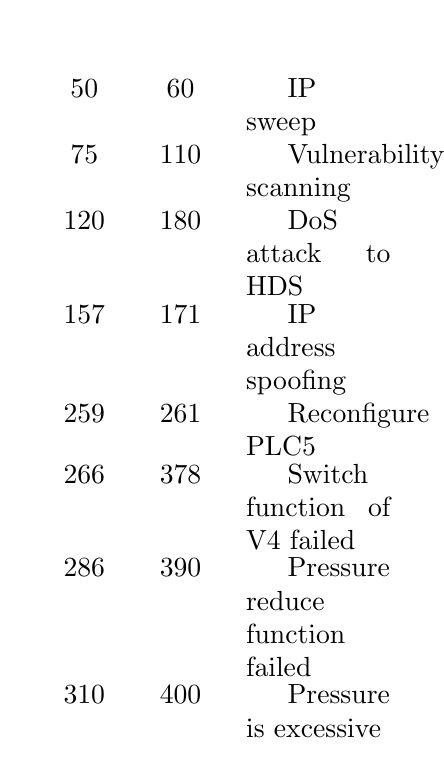
\begin{tikzpicture}[line width = 1pt]
\taburowcolors[2] 2{black!10 .. black!30}

\node at (0,0) {
\begin{tabu} to 4.7cm{*2{X[c,-1]|[1.5pt white]}X[l]}
\rowcolor{black!80}\rowfont\bfseries \textcolor{white}{Start}  & \textcolor{white}{End} & \textcolor{white}{Description}\\\tabucline[1.5pt white]{-}
50            & 60        & IP sweep                          \\\tabucline[1.5pt white]{-}
75            & 110       & Vulnerability scanning            \\\tabucline[1.5pt white]{-}
120           & 180       & DoS attack to HDS                 \\\tabucline[1.5pt white]{-}
157           & 171       & IP address spoofing               \\\tabucline[1.5pt white]{-}
259           & 261       & Reconfigure PLC5                  \\\tabucline[1.5pt white]{-}
266           & 378       & Switch function of V4 failed      \\\tabucline[1.5pt white]{-}
286           & 390       & Pressure reduce function failed   \\\tabucline[1.5pt white]{-}
310           & 400       & Pressure is excessive             \\

\end{tabu}
};
\end{tikzpicture}

}};


\draw[-{>[scale = 0.5, length=5, width = 6]}] (0.2,5.75) -- (1.5,5.75) node [midway, above] {Trigger};
\draw[{<[scale = 0.5, length=5, width = 6]}-{>[scale = 0.5, length=5, width = 6]}, line width = 0.5pt] (0.4, 4.9) -- (1.2, 4.9) node [midway, fill = white, rotate = 45, inner sep = 1pt] {\fontsize{4pt}{4pt}\selectfont 1 min};
\draw[line width = 0.5pt] (0.2,5.6) -- (0.4, 5.6) -- (0.4,5.2) -- (0.8,5.2) -- (0.8,5.6) -- (1.2, 5.6) -- (1.2,5.2) -- (1.4,5.2);
\draw[line width = 0.5pt] (0.4, 4.7) -- (0.4, 5.1);
\draw[line width = 0.5pt] (1.2, 4.7) -- (1.2, 5.1);

\draw[-{>[scale = 0.5, length=5, width = 6]}] (5.5, 6.5) -- (7, 6.5) node [midway, sloped, align = center] {Attack\\ Evidence};

\draw[-{>[scale = 0.5, length=5, width = 6]}] (5.5, 5) -- (7, 5) node [midway, sloped, align = center] {Anomaly\\ Evidence};

\draw[white, line width = 3pt] (19.6, 5.75) -- (20.4,5.75);
\foreach \y/\t in {1/x_1,
				   2/x_2,
				   3/x_3,
				   4/x_4,
				   5/x_5,
				   6/x_6,
				   7/x_7,
				   8/x_8}{
	\node (t\y) at (15 + 0.5*\y, 8-0.5*\y) [circle, fill = black, inner sep = 0pt, minimum size = 0.15cm] {\textcolor[rgb]{1,1,1}{\scalebox{0.5}{$\bm{\times}$}}};
	\draw[white, line width = 1.5pt] (13, 8 - 0.5*\y) -- (t\y);
	\fill (13 + 0.2*\y, 8 - 0.5*\y) circle (0.05cm);
	\draw[-{>[scale = 0.5, length=5, width = 6]}] (13 + 0.2*\y, 8 - 0.5*\y) -- (13 + 0.2*\y, 0.7 + 0.2*\y) -- (15.5, 0.7 0+ 0.2*\y);
	
	\node at (12, 8 - 0.5*\y - 0.1) [anchor = south west] {$p(\t)$};
		
	\draw[-{>[scale = 0.5, length=5, width = 6]}] (12, 8 - 0.5*\y) -- (t\y);
	\draw[-{>[scale = 0.5, length=5, width = 6]}] (t\y) -- (19.4, 8 - 0.5*\y);
	\draw[-{>[scale = 0.5, length=5, width = 6]}] (15 + 0.5*\y, 3.6) -- (t\y);
	\node at (15 + 0.5*\y, 3.45) [rotate = 45] {$q(\t)$};
	
	\fill (19.4,3.8) rectangle (19.8,7.7) ;
}


\draw[-{>[scale = 0.5, length=5, width = 6]}] (19.5, 5.75) -- (20.8,5.75) node [below left= -7pt and -1pt] {Risk};
\node at (19.6,5.75) {\textcolor[rgb]{1,1,1}{$\sum$}};

\fill[black] (15.5, 0.7) rectangle (15.7,2.5);
\node at (15.6, 2.7) {Mux};

\draw[-{>[scale = 0.5, length=5, width = 6]}] (15.7, 1.6) -- (16.5, 1.6);

\myscope{16.5}{1.6}
\myscope{20.8}{5.75}

\foreach \x/\i/\e/\t in {0/1/x_{1}/Product damaged,
					     0/2/x_{2}/Tank damaged,
					     0/3/x_{3}/Heater damaged,
					     0/4/x_{4}/Sensors damaged,
					     1/1/x_{5}/Staff$_{1\text{-}4}$ injured,
					     1/2/x_{6}/Staff$_{5\text{-}9}$ injured,
					     1/3/x_{7}/Water pollution,
					     1/4/x_{8}/Air pollution}{
	\node at (5.2 + 4*\x + 0.7, 2.9 - 0.5*\i) [anchor = east] {$\e$};
	\node at (5.2 + 4*\x + 0.5, 2.9 - 0.5*\i) [anchor = west] {-- \t};
}

\foreach \i/\c/\t in {1/attack/Attack node,
					  2/resource/Resource node,
					  3/function/Function node,
					  4/incident/Incident node}{
	%\fill[\c] (2,2.9 - 0.5*\i) circle (0.12cm);
    \node[\c] at (1.7,2.9 - 0.5*\i){};
	\node at (1.9,2.9 - 0.5*\i) [anchor = west] {\t};
}


\end{tikzpicture}

    \end{center}
\end{frame}

\begin{frame}{Simulation Platform}
    \label{Simulation: Multi-Level Bayesian Network of Reactor}
    The multi-level Bayesian network of the chemical reactor is shown as following figure.\vspace{-18pt}\\
    \begin{center}
      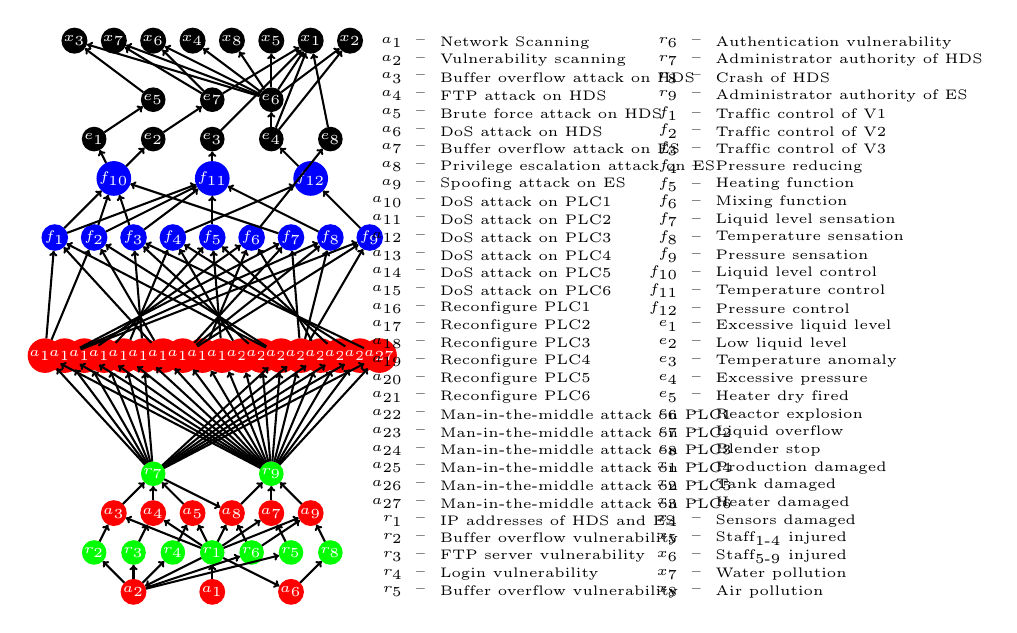
\begin{tikzpicture}[line width = \pgfdefaultlinewidth,
                    x = 0.25cm,
                    y = 0.25cm,
					attack/.style = {draw = red, fill = red, text = white, circle, minimum size = 0.2cm, inner sep=0pt},
					resource/.style = {draw = green, fill = green, text = white, circle, minimum size = 0.2cm, inner sep=0pt},
					function/.style = {draw = blue, fill = blue, text = white, circle, minimum size = 0.2cm, inner sep=0pt},
					incident/.style = {draw = black, circle, fill = black, text = white, minimum size = 0.2cm, inner sep=0pt},
					auxiliary/.style = {draw = black, circle, fill = black, text = white, minimum size = 0.2cm, inner sep=0pt},
                    arrow/.style = {-{>[scale = 0.5, length=4, width = 6]}}]

\fontsize{3pt}{3pt}\selectfont

\node[attack]    (a1) at (12,  1) {$a_1$};
\node[attack]    (a2) at ( 8,  1) {$a_2$};
\node[attack]    (a6) at (16,  1) {$a_6$};

\foreach \i/\x in {2/6,
				   3/8,
				   4/10,
				   1/12,
				   6/14,
				   5/16,
				   8/18}{
	\node[resource] (r\i) at (\x, 3) {$r_{\i}$};
}

\foreach \i/\x in {3/7,
				   4/9,
				   5/11,
				   8/13,
				   7/15,
				   9/17}{
	\node[attack] (a\i) at (\x, 5) {$a_{\i}$};
}

\foreach \i/\x in {7/9,
				   9/15}{
	\node[resource] (r\i) at (\x, 7) {$r_{\i}$};
}

\foreach \i in {10,...,27}{
	\node[attack] (a\i) at (\i - 6.5, 13) {$a_{\i}$};
}

\foreach \i in {1,...,9}{
	\node[function] (f\i) at (2 + 2*\i, 19) {$f_{\i}$};
}

\foreach \i/\x in {10/7,
				   11/12,
				   12/17}{
	\node[function] (f\i) at (\x, 22) {$f_{\i}$};
}

\foreach \i/\x in {1/6,
				   2/9,
				   3/12,
				   4/15,
				   8/18}{
	\node[incident] (e\i) at (\x, 24) {$e_{\i}$};
}

\foreach \i/\x in {5/9,
				   7/12,
				   6/15}{
	\node[incident] (e\i) at (\x, 26) {$e_{\i}$};
}

\foreach \i/\x in {3/5,
				   7/7,
				   6/9,
				   4/11,
				   8/13,
				   5/15,
				   1/17,
				   2/19}{
	\node[incident] (x\i) at (\x, 29) {$x_{\i}$};
}


\foreach \i/\j in{a1/r1,
                  r1/a2,
                  r1/a6,
                  r1/a3,
                  r1/a4,
                  r1/a5,
                  r1/a7,
                  r1/a8,
                  r1/a9,
                  a2/r2,
                  a2/r3,
                  a2/r4,
                  a2/r5,
                  a2/r6,
                  r2/a3,
                  r3/a4,
                  r4/a5,
                  r5/a7,
                  r6/a8,
                  r6/a9,
                  a6/r8,
                  r8/a9,
                  a3/r7,
                  a4/r7,
                  a5/r7,
                  a7/r9,
                  r7/a8,
                  r7/a10,
                  r7/a11,
                  r7/a12,
                  r7/a13,
                  r7/a14,
                  r7/a15,
                  r7/a22,
                  r7/a23,
                  r7/a24,
                  r7/a25,
                  r7/a26,
                  r7/a27,
                  a8/r9,
                  a9/r9,
                  r9/a10,
                  r9/a11,
                  r9/a12,
                  r9/a13,
                  r9/a14,
                  r9/a15,
                  r9/a16,
                  r9/a17,
                  r9/a18,
                  r9/a19,
                  r9/a20,
                  r9/a21,
                  r9/a22,
                  r9/a23,
                  r9/a24,
                  r9/a25,
                  r9/a26,
                  r9/a27,
                  a10/f1,
                  a10/f2,
                  a11/f7,
                  a11/f8,
                  a11/f9,
                  a12/f6,
                  a13/f5,
                  a14/f4,
                  a15/f3,
                  a16/f1,
                  a16/f2,
                  a17/f7,
                  a17/f8,
                  a17/f9,
                  a18/f6,
                  a19/f5,
                  a20/f4,
                  a21/f3,
                  a22/f1,
                  a22/f2,
                  a23/f7,
                  a23/f8,
                  a23/f9,
                  a24/f6,
                  a25/f5,
                  a26/f4,
                  a27/f3,
                  f1/f10,
                  f1/f11,
                  f2/f10,
                  f2/f11,
                  f3/f10,
                  f3/f11,
                  f4/f12,
                  f5/f11,
                  f6/e8,
                  f7/f10,
                  f8/f11,
                  f9/f12,
                  f10/e1,
                  f10/e2,
                  f11/e3,
                  f12/e4,
                  e1/e5,
                  e2/e7,
                  e3/x1,
                  e4/e6,
                  e4/x1,
                  e4/x2,
                  e5/x3,
                  e6/x1,
                  e6/x2,
                  e6/x3,
                  e6/x4,
                  e6/x5,
                  e6/x6,
                  e6/x7,
                  e6/x8,
                  e7/x1,
                  e7/x6,
                  e7/x7,
                  e8/x1}{
	\draw[arrow] (\i) -- (\j);
}

\foreach \i/\c/\n/\e in { 1/1/a_{ 1}/Network Scanning,
                          2/1/a_{ 2}/Vulnerability scanning,
                          3/1/a_{ 3}/Buffer overflow attack on HDS,
                          4/1/a_{ 4}/FTP attack on HDS,
                          5/1/a_{ 5}/Brute force attack on HDS,
                          6/1/a_{ 6}/DoS attack on HDS ,
                          7/1/a_{ 7}/Buffer overflow attack on ES,
                          8/1/a_{ 8}/Privilege escalation attack on ES,
                          9/1/a_{ 9}/Spoofing attack on ES,
                         10/1/a_{10}/DoS attack on PLC1,
                         11/1/a_{11}/DoS attack on PLC2,
                         12/1/a_{12}/DoS attack on PLC3,
                         13/1/a_{13}/DoS attack on PLC4,
                         14/1/a_{14}/DoS attack on PLC5,
                         15/1/a_{15}/DoS attack on PLC6,
                         16/1/a_{16}/Reconfigure PLC1,
                         17/1/a_{17}/Reconfigure PLC2,
                         18/1/a_{18}/Reconfigure PLC3,
                         19/1/a_{19}/Reconfigure PLC4,
                         20/1/a_{20}/Reconfigure PLC5,
                         21/1/a_{21}/Reconfigure PLC6,
                         22/1/a_{22}/Man-in-the-middle attack on PLC1,
                         23/1/a_{23}/Man-in-the-middle attack on PLC2,
                         24/1/a_{24}/Man-in-the-middle attack on PLC3,
                         25/1/a_{25}/Man-in-the-middle attack on PLC4,
                         26/1/a_{26}/Man-in-the-middle attack on PLC5,
                         27/1/a_{27}/Man-in-the-middle attack on PLC6,
                         28/1/r_{ 1}/IP addresses of HDS and ES,
                         29/1/r_{ 2}/Buffer overflow vulnerability,
                         30/1/r_{ 3}/FTP server vulnerability,
                         31/1/r_{ 4}/Login vulnerability,
                         32/1/r_{ 5}/Buffer overflow vulnerability,
                         33/2/r_{ 6}/Authentication vulnerability,
                         34/2/r_{ 7}/Administrator authority of HDS,
                         35/2/r_{ 8}/Crash of HDS,
                         36/2/r_{ 9}/Administrator authority of ES,
                         37/2/f_{ 1}/Traffic control of V1,
                         38/2/f_{ 2}/Traffic control of V2,
                         39/2/f_{ 3}/Traffic control of V3,
                         40/2/f_{ 4}/Pressure reducing,
                         41/2/f_{ 5}/Heating function,
                         42/2/f_{ 6}/Mixing function,
                         43/2/f_{ 7}/Liquid level sensation,
                         44/2/f_{ 8}/Temperature sensation,
                         45/2/f_{ 9}/Pressure sensation,
                         46/2/f_{10}/Liquid level control,
                         47/2/f_{11}/Temperature control,
                         48/2/f_{12}/Pressure control,
                         49/2/e_{ 1}/Excessive liquid level,
                         50/2/e_{ 2}/Low liquid level,
                         51/2/e_{ 3}/Temperature anomaly,
                         52/2/e_{ 4}/Excessive pressure,
                         53/2/e_{ 5}/Heater dry fired,
                         54/2/e_{ 6}/Reactor explosion,
                         55/2/e_{ 7}/Liquid overflow,
                         56/2/e_{ 8}/Blender stop,
                         57/2/x_{ 1}/Production damaged,
                         58/2/x_{ 2}/Tank damaged,
                         59/2/x_{ 3}/Heater damaged,
                         60/2/x_{ 4}/Sensors damaged,
                         61/2/x_{ 5}/Staff$_{\text{1-4}}$ injured,
                         62/2/x_{ 6}/Staff$_{\text{5-9}}$ injured,
                         63/2/x_{ 7}/Water pollution,
                         64/2/x_{ 8}/Air pollution}{
	\node[anchor = east] at (9.2 + 14*\c, 1 - 0.9*\i + 28.8*\c) {\tiny $\n$ \ -- };
	\node[anchor = west] at (9.2 + 14*\c, 1 - 0.9*\i + 28.8*\c) {\tiny \e};
}
\end{tikzpicture}

    \end{center}
\end{frame}

\begin{frame}{Simulation Platform}
    \label{Simulation: Evidences List}
    The list of evidences is shown as following table.

    \taburowcolors[2] 2{black!10 .. black!30}
    \extrarowsep = 1mm
    \begin{tabu} to \textwidth{*2{X[c,-1]|[1.5pt white]}X[l]|[1.5pt white]X[-1, c]}
    \rowcolor{black!80}\rowfont\bfseries \textcolor{white}{Start}  & \textcolor{white}{End} & \textcolor{white}{Description} & \textcolor{white}{Symbol}\\\tabucline[1.5pt white]{-}
    50            & 60        & IP sweep                         & $L(a_1)$ \\\tabucline[1.5pt white]{-}
    75            & 110       & Vulnerability scanning           & $L(a_2)$ \\\tabucline[1.5pt white]{-}
    120           & 180       & DoS attack to HDS                & $L(a_6)$ \\\tabucline[1.5pt white]{-}
    157           & 171       & IP address spoofing              & $L(a_9)$ \\\tabucline[1.5pt white]{-}
    259           & 261       & Reconfigure PLC5                 & $L(a_{20})$ \\\tabucline[1.5pt white]{-}
    266           & 378       & Switch function of V4 failed     & $F(f_4)$ \\\tabucline[1.5pt white]{-}
    286           & 390       & Pressure reduce function failed  & $F(f_{12})$ \\\tabucline[1.5pt white]{-}
    310           & 400       & Pressure is excessive            & $H(e_4)$ \\

    \end{tabu}
\end{frame}

\begin{frame}{Simulation Platform}
    \label{Simulation: Quantification of Consequences}
    The quantification of consequences is shown as following table.

    \newcolumntype Z{X[m, c, 1.8]{%
    S[
    %group-four-digits=true ,
    round-mode = figures,
    group-separator = {,},
    add-decimal-zero = false,
    round-integer-to-decimal=true ,
    table-number-alignment = center,
    table-space-text-pre = \hspace{30pt},
    per-mode=symbol]}}
    \tabucolumn Z
    \taburowcolors[2] 2{black!10 .. black!30}
    \tabulinesep = 1mm
    \extrarowsep = 1mm
    \begin{tabu}to \textwidth{X[c,1, m]|[1.5pt white]X[m, 3]|[1.5pt white]Z}

    \rowcolor{black!80}\rowfont\bfseries
        \textcolor{white}{Incident Symbol} &
        \textcolor{white}{Description of Incident} &
        \textcolor{white}{\bf Quantification of Consequence(\$)}\\
    \tabucline[1.5pt white]{-}
        $x_{1}$  & Product damaged              & 50000  \\\tabucline[1.5pt white]{-}
        $x_{2}$  & Tank damaged                 & 500000 \\\tabucline[1.5pt white]{-}
        $x_{3}$  & Heater damaged               & 10000  \\\tabucline[1.5pt white]{-}
        $x_{4}$  & Sensors damaged              & 10000  \\\tabucline[1.5pt white]{-}
        $x_{5}$  & Staff$_{\text{1-4}}$ injured & 800000 \\\tabucline[1.5pt white]{-}
        $x_{6}$  & Staff$_{\text{5-9}}$ injured & 1000000\\\tabucline[1.5pt white]{-}
        $x_{7}$  & Water pollution              & 200000 \\\tabucline[1.5pt white]{-}
        $x_{8}$  & Air pollution                & 200000 \\
    \end{tabu}
\end{frame}

\subsection{Simulation and Result Analysis}
\begin{frame}{Simulation and Result Analysis}
    \label{Simulation: Curvers of Cybersecurity Risk and Incident Probability}
    \begin{center}
      ��\begin{tikzpicture}
    \tikzset{
        every pin/.style={pin distance=3pt, font = \small},
        small dot/.style={fill=black,circle,scale=0.3}
    }
    \begin{axis}[height             = 4cm,
                 width              = \textwidth,
                 ylabel             = Risk,
                 xlabel             = Absolute Time(Min),
                 x label style      = 
                 {
                    font            = \footnotesize, 
                    at              = {(0.5, 0.06)}
                 },
                 y label style      = 
                 {
                    font            = \footnotesize, 
                    at              = {(0.05, 0.5)}},
                    enlargelimits   = false,
                 label style        = 
                 {
                    font            = \footnotesize
                 },
                 legend style       = 
                 {
                    legend pos      = north west,
                    font            = \footnotesize
                 },
                 legend cell align  = left]
                 
        \addplot [solid,  line width = 1pt, red]   file {Data/RiskWithKnowledge.dat};

        \node[fill=black,circle,scale=0.3,pin=above:{$a_1$}]                at (axis cs:5.0000000e+01,4.1401694e+04) {};
        \node[fill=black,circle,scale=0.3,pin=above:{$a_2$}]                at (axis cs:7.5000000e+01,8.2803359e+04) {};
        \node[fill=black,circle,scale=0.3,pin=above:{$a_6$}]                at (axis cs:1.2000000e+02,1.0997221e+05) {};
        \node[fill=black,circle,scale=0.3,pin=above:{$a_9$}]                at (axis cs:1.5700000e+02,1.5891921e+05) {};
        \node[fill=black,circle,scale=0.3,pin=135:  {$a_{20}$}]             at (axis cs:2.5900000e+02,2.3773019e+05) {};
        \node[fill=black,circle,scale=0.3,pin=above:{$f_4$}]                at (axis cs:2.6600000e+02,3.6620292e+05) {};
        \node[fill=black,circle,scale=0.3,pin=-45:  {$f_{12}$}]             at (axis cs:2.8600000e+02,5.9882195e+05) {};
        \node[fill=black,circle,scale=0.3,pin=-45:  {$e_4$}]                at (axis cs:3.1000000e+02,8.6217598e+05) {};
        \node[fill=black,circle,scale=0.3,pin=-135: {$\overline{f}_4$}]     at (axis cs:3.7800000e+02,8.6333260e+05) {};
        \node[fill=black,circle,scale=0.3,pin=-90:  {$\overline{f}_{12}$}]  at (axis cs:3.9000000e+02,8.6333260e+05) {};
        \node[fill=black,circle,scale=0.3,pin=180:  {$\overline{e}_4$}]     at (axis cs:4.0000000e+02,2.3773019e+05) {};
        \node[fill=black,circle,scale=0.3,pin=135:  {Attack timeout}]       at (axis cs:4.1200000e+02,1.1416258e-01) {};
    \end{axis}
\end{tikzpicture} \\
      ��\begin{tikzpicture}
    \begin{axis}[height             = 4cm,
                 width              = \textwidth,
                 ylabel             = Probability,
                 xlabel             = Absolute Time(Min),
                 x label style      =
                 {                  
                    font            = \footnotesize,
                    at              = {(0.5, 0.06)}
                 },                 
                 y label style      =
                 {                  
                    font            = \footnotesize,
                    at              = {(0.05, 0.5)}
                 },                 
                 scaled y ticks     = {base 10:1},
                 enlargelimits      = false,
                 label style        =
                 {                  
                    font            = \footnotesize
                 },                 
                 legend style       =
                 {                  
                    legend pos      = north west,
                    font            = \tiny,
                    column sep      = 5pt
                 },
                 legend cell align  = left,
                 legend columns     = 2]

        \addplot [solid,          line width = \pgfdefaultlinewidth, black] file {Data/px1.dat};
        \addplot [densely dotted, line width = \pgfdefaultlinewidth, black] file {Data/px2.dat};
        \addplot [dashed,         line width = \pgfdefaultlinewidth, black] file {Data/px3.dat};
        \addplot [solid,          line width = \pgfdefaultlinewidth, blue]  file {Data/px4.dat};
        \addplot [densely dotted, line width = \pgfdefaultlinewidth, blue]  file {Data/px5.dat};
        \addplot [dashed,         line width = \pgfdefaultlinewidth, blue]  file {Data/px6.dat};
        \addplot [solid,          line width = \pgfdefaultlinewidth, red]   file {Data/px7.dat};
        \addplot [densely dotted, line width = \pgfdefaultlinewidth, red]   file {Data/px8.dat};

        \scriptsize
        \legend {Product damaged,
                 Tank damaged,
                 Heater damaged,
                 Sensors damaged,
                 $\text{Staff}_{\text{1-4}}$ injured,
                 $\text{Staff}_{\text{5-9}}$ injured,
                 Water polluted,
                 Air polluted};
    \end{axis}
\end{tikzpicture} \\
    \end{center}
\end{frame}

\begin{frame}{Simulation and Result Analysis}
    \label<trans:1>{Simulation: Ability to Deal with the Unknown Attacks Step 1}
    \label<trans:2>{Simulation: Ability to Deal with the Unknown Attacks Step 2}
    \label<trans:3>{Simulation: Ability to Deal with the Unknown Attacks Step 3}
    \vspace{10pt}
    \begin{overlayarea}{\textwidth}{1cm}
        \only<1| trans:1>{In the previous simulation, the curve of the cybersecurity risk is shown as the \textcolor{red}{\bf red} line in the following figure.}
        \only<2| trans:2>{To validate the ability to deal with the unknown attacks, the attack knowledge about attack \textcolor{red}{\st{$a_6$}} and attack \textcolor{red}{\st{$a_9$}} is removed from the multi-level Bayesian network.}
        \only<3| trans:3>{Then an identical multi-step attack on the system is launched to the system. The new cybersecurity risk curve is shown the dashed line in the following figure.}
    \end{overlayarea}\vspace{10pt}
    \begin{center}
      ��\begin{tikzpicture}
    \tikzset{
        every pin/.style            =
        {
            pin distance            = 3pt,
            font                    = \small
        },
        small dot/.style            =
        {
            fill                    = black,
            circle,
            scale                   = 0.3
        }
    }
    \begin{axis}[height             = 6cm,
                 width              = \textwidth,
                 ylabel             = Risk,
                 xlabel             = Absolute Time(Min),
                 enlargelimits      = false,
                 x label style      =
                 {
                    font            = \footnotesize,
                    at              = {(0.5, 0)}
                 },
                 y label style      =
                 {
                    font            = \footnotesize,
                    at              = {(0.05, 0.5)}
                 },
                 legend style       =
                 {
                    legend pos      = north west,
                    font            = \scriptsize
                 },
                 legend cell align  = left]

        \addplot [solid,  line width = 0.5pt, red]   file {Data/RiskWithKnowledge.dat};
        \only<3| trans:3>{
            \addplot [dashed, line width = 1pt, black]   file {Data/RiskWithoutKnowledge.dat};
        }

        \node[fill=black,circle,scale=0.3,pin=above:{$a_1$}]                at (axis cs:5.0000000e+01,4.1401694e+04) {};
        \node[fill=black,circle,scale=0.3,pin=above:{$a_2$}]                at (axis cs:7.5000000e+01,8.2803359e+04) {};
        \node[fill=black,circle,scale=0.3,pin=above:{
            \temporal<2| trans:2>{$a_6$}{\textcolor{red}{\st{$a_6$}}}{\textcolor{red}{\st{$a_6$}}}
        }]                at (axis cs:1.2000000e+02,1.0997221e+05) {};
        \node[fill=black,circle,scale=0.3,pin=above:{
            \temporal<2| trans:2>{$a_9$}{\textcolor{red}{\st{$a_9$}}}{\textcolor{red}{\st{$a_9$}}}
        }]                at (axis cs:1.5700000e+02,1.5891921e+05) {};
        \node[fill=black,circle,scale=0.3,pin=135:  {$a_{20}$}]             at (axis cs:2.5900000e+02,2.3773019e+05) {};
        \node[fill=black,circle,scale=0.3,pin=above:{$f_4$}]                at (axis cs:2.6600000e+02,3.6620292e+05) {};
        \node[fill=black,circle,scale=0.3,pin=-45:  {$f_{12}$}]             at (axis cs:2.8600000e+02,5.9882195e+05) {};
        \node[fill=black,circle,scale=0.3,pin=-85:  {$e_4$}]                at (axis cs:3.1000000e+02,8.6217598e+05) {};
        \node[fill=black,circle,scale=0.3,pin=-135: {$\overline{f}_4$}]     at (axis cs:3.7800000e+02,8.6333260e+05) {};
        \node[fill=black,circle,scale=0.3,pin=-90:  {$\overline{f}_{12}$}]  at (axis cs:3.9000000e+02,8.6333260e+05) {};
        \node[fill=black,circle,scale=0.3,pin=180:  {$\overline{e}_4$}]     at (axis cs:4.0000000e+02,2.3773019e+05) {};
        \node[fill=black,circle,scale=0.3,pin=135:  {Attack timeout}]       at (axis cs:4.1200000e+02,1.1416258e-01) {};

        \only<3| trans:3>{
            \addlegendentry[align=left]{Risk assessment with all\\ attack knowledge}
            \addlegendentry[align=left]{Risk assessment without\\ knowledge about $a_6$ and $a_9$}
        }
    \end{axis}
\end{tikzpicture} 
    \end{center}
\end{frame}

\begin{frame}{Simulation and Result Analysis}
    \label<trans:1>{Simulation: Curve of Execution Time Distribution Step 1}
    \label<trans:2>{Simulation: Curve of Execution Time Distribution Step 2}
    \label{Simulation: Curve of Execution Time Distribution}
    \vspace{10pt}
    \begin{overlayarea}{\textwidth}{1.8cm}
        \only<1| trans:1>{We repeat the first simulation 5,000 times, and the execution time of 5,000 calculations is recorded. This simulation is run on a machine with Intel Pentium processor G3220 (3M Cache, 3.00GHz) and 4GB DDR3 memory. The following figure shows the distribution of the 5,000 execution times.}
        \only<2-| trans:2>{Some parameters of the following figure:
        \begin{itemize}
           \item<2-> The average execution time of a risk assessment is $94.1$ms.
           \item<3-> The minimum execution time of a risk assessment is $89.9$ms.
           \item<4-> The maximum execution time of a risk assessment is $131.6$ms.
         \end{itemize}}
    \end{overlayarea}\vspace{10pt}
    \begin{center}
      ��\begin{tikzpicture}
    \begin{groupplot}[anchor      = north west,
                      group style = {
                          group name     = coupeplot,
                          group size     = 2 by 1,
                          yticklabels at = edge left,
                          horizontal sep = 0pt
                      },
                      ymin        = 0,
                      ymax        = 0.07]
        \nextgroupplot[ybar,
                       bar width        = 0.13cm,
                       bar shift        = 0pt,
                       xmin             = 0.09,
                       xmax             = 0.1,
                       xtick            = {0.09,0.095,0.1},
                       axis y line*     = left,
                       height           = 5cm,
                       width            = 0.8\textwidth,
                       ylabel           = Probability,
                       xlabel           = Execution Time,
                       xticklabel style = {/pgf/number format/.cd,fixed,precision=5, fixed zerofill, precision=3},
                       every axis y label/.append style = {at={(0.089, 0.5)}},
                       every axis x label/.append style = {at={(0.6, 0)}}]
        \addplot[fill = black, draw = none] file {Data/DistributionExecutionTime.dat};  				
        \nextgroupplot[ybar,
                       bar width        = 0.13cm,
                       bar shift        = 0pt,
                       xmin             = 0.13,
                       xmax             = 0.132,
                       axis x discontinuity = crunch,
                       xtick            = {0.132},
                       axis y line*     = right,
                       xticklabel style = {/pgf/number format/.cd,fixed,precision=5, fixed zerofill, precision=3},
                       height           = 5cm,
                       width            = 0.3\textwidth]
        \pgfplotsset{cycle list shift=+1}
        \addplot[fill = black] coordinates{(1.3153017e-01, 1.0001000e-04)};
    \end{groupplot}
\end{tikzpicture}
    \end{center}
\end{frame}

\begin{frame}{Simulation and Result Analysis}
    \label<trans:1>{Simulation: Curves of Risk Assessment Algorithm Scalability Step 1}
    \label<trans:2>{Simulation: Curves of Risk Assessment Algorithm Scalability Step 2}
    \label<trans:3>{Simulation: Curves of Risk Assessment Algorithm Scalability Step 3}
    \vspace{10pt}
    \begin{overlayarea}{\textwidth}{1.8cm}
    \only<1| trans:1>{Finally, 25 multi-level Bayesian networks with different node sizes are adopted to show the possible upper/lower bounds and the scalability of our approach.}
    \only<2| trans:2>{In the following figure, the fitting line $$y = 0.0019x - 0.0175$$ matches well with the correlation coefficient $r = 0.9987$.}
    \only<3| trans:3>{This means that the execution time of the risk assessment scales linearly with the increase of the node size of the multi-level Bayesian network.}
    \end{overlayarea}\vspace{10pt}
    \begin{center}
      ��\begin{tikzpicture}
    \begin{axis}[height           = 6cm,
                 width            = \textwidth,
                 ylabel           = Execution Time (s),
                 xlabel           = Number of Nodes,
                 label style      = {font = \footnotesize},
                 xticklabel style = {/pgf/number format/.cd,fixed, fixed zerofill, precision=0},
                 x label style = {font = \footnotesize, at={(0.5, 0.02)}},
                 y label style = {font = \footnotesize, at={(0.04, 0.5)}},
                 enlargelimits    = false,
                 legend style     ={legend pos=north west,font=\scriptsize},
                 legend cell align=left
                ]
        \addplot[draw = none, name path = Max, forget plot] file {Data/MaxCalculationTime.dat};
        \addplot[draw = none, name path = Min, forget plot] file {Data/MinCalculationTime.dat};
        \addplot[black!50] fill between[of= Min and Max];
        \addplot[only marks, mark size=1pt] file {Data/AverCalculationTime.dat};
        \only<1| trans:1>{\addplot[line width = 0.7pt, domain=10:490] {0.0019*x - 0.0175};}
        \only<2-| trans:2->{\addplot[line width = 0.7pt, domain=10:490, red] {0.0019*x - 0.0175} node [pos=0.5, below, sloped, red] {$y = 0.0019x - 0.0175$};}


        \legend {Scope between upper and lower bounds,
                 Average execution time of risk assessment,
                 Best fitting line of average execution time};

    \end{axis}
\end{tikzpicture} 
    \end{center}
\end{frame}


\section{Conclusion and Prospect}
\subsection{Conclusion}
\begin{frame}{Conclusion}
\begin{itemize}[<+->]
  \item By considering the characteristics of ICSs, a novel multi-level Bayesian network was proposed, which integrated a knowledge of attack, system function, and hazardous incident.
  \item The attack knowledge and system knowledge were combined to analyze the potential impact of attacks, so the proposed approach had the ability of assessing the risk caused by unknown attacks.
  \item A unified quantification approach for a variety of consequences of industrial accidents was introduced. Furthermore, the proposed approach could eliminate the error of risk caused by the overlapping amongst hazardous incidents.
  \item By using a simplified chemical reactor control system in Matlab environment, the designed dynamic risk assessment approach was verified.
\end{itemize}
\end{frame}

\subsection{Prospect}
\begin{frame}{Prospect}
    There are some shortcomings of the proposed risk assessment approach need to be improved.
    \begin{itemize}[<+->]
      \item \textbf{Current research work has no ability for self-learning.} 
      \item \textbf{The sub-second computation time cannot meet some hard real-time systems requirements.}
    \end{itemize}
    \uncover<+->{In the future, a dynamic cybersecurity risk assessment, which can automatically adjust the conditional probability and structure of the multi-level Bayesian network by analyzing the real-time data, will be researched, and several approximate inference methods will be attempted in the risk assessment.}
\end{frame}


% Thank You!
\setbeamercolor{background canvas}{bg=mDarkTeal}
\begin{frame}{}
    \label{Section: Thank You}
    \centering
    \vfill\vspace{1em}\usebeamerfont{section title}\textcolor{white}{\scshape Thank You!}\vfill
\end{frame}

\setbeamercolor{background canvas}{bg=white}

\begin{frame}{Thank You!}
    \label{Thank You: Thank You}
    You can obtain this slide from my Github:\\
    \href{https://github.com/zqmillet/Presentation.for.Loughborough.University}{\tt \small \textcolor{blue}{zqmillet@github.com:Presentation.for.Loughborough.University}}\\[15pt]

    \pause
    And I have pushed the code of the simulation to my Github, too.\\
    \href{https://github.com/zqmillet/Multi-level.Bayesian.Network}{\tt \small \textcolor{blue}{zqmillet@github.com:Multi-level.Bayesian.Network}}\\[15pt]

\end{frame}

% Questions
\setbeamercolor{background canvas}{bg=mDarkTeal}
\begin{frame}{}
    \label{Section: Questions}
    \centering
    \vfill\vspace{1em}\usebeamerfont{section title}\textcolor{white}{\scshape Any Questions?}\vfill
\end{frame}



\end{document}
